%% =====================================================================
%% CivicSight -- Final Report (revised), SINGLE-FILE version.
%% Generated by scripts/flatten_tex.py from main.tex, chapters/, diagrams/ and
%% civicsight-style.sty. Needs only tietreport.cls, references.bib and figures/
%% in the same folder. Compile: pdfLaTeX -> Biber -> pdfLaTeX -> pdfLaTeX.
%% =====================================================================
%% =====================================================================
%% CivicSight -- Final (End-Semester) Software Engineering Project Report
%% Revised edition (condensed). Built on the official TIET template:
%% tietreport.cls is an unmodified copy; chapter/section order follows the template main.tex.
%% Compile with: pdfLaTeX -> Biber -> pdfLaTeX -> pdfLaTeX (Overleaf does this automatically)
%% =====================================================================
\documentclass[openany]{tietreport}

% Report styling: colours, headings, tables, TikZ diagram styles
%% ---- begin civicsight-style.sty (inlined) ----
\makeatletter
%% civicsight-style.sty
%% Visual styling for the CivicSight final report.
%% Loaded on top of the official tietreport.cls (which is left unmodified).

%% ---------------------------------------------------------------
%% Packages
%% ---------------------------------------------------------------
\RequirePackage[T1]{fontenc}
\RequirePackage[utf8]{inputenc}
\RequirePackage{lmodern}
\RequirePackage[scaled=0.92]{helvet}
\RequirePackage{microtype}
\RequirePackage[table,dvipsnames]{xcolor}
\RequirePackage{booktabs}
\RequirePackage{tabularx}
\RequirePackage{array}
\RequirePackage{longtable}
\RequirePackage{multirow}
\RequirePackage{makecell}
\RequirePackage{float}
\RequirePackage{caption}
\RequirePackage{subcaption}
\RequirePackage{enumitem}
\RequirePackage{tikz}
\RequirePackage{pifont}
\RequirePackage[most]{tcolorbox}
\RequirePackage{listings}
\RequirePackage{needspace}
\RequirePackage{adjustbox}
\setlength{\emergencystretch}{3em}
\usetikzlibrary{positioning,arrows.meta,shapes.geometric,shapes.multipart,
  shapes.misc,fit,calc,backgrounds,matrix,decorations.pathreplacing}

%% ---------------------------------------------------------------
%% Colour palette (restrained: navy / teal / terracotta / sand)
%% ---------------------------------------------------------------
\definecolor{csNavy}{HTML}{1B3A5C}
\definecolor{csTeal}{HTML}{2F7F7A}
\definecolor{csTerra}{HTML}{C2603A}
\definecolor{csSand}{HTML}{D8A657}
\definecolor{csSlate}{HTML}{6B7A8F}
\definecolor{csInk}{HTML}{1F2933}
\definecolor{csLine}{HTML}{9AA5B1}
\definecolor{csLight}{HTML}{F3F5F7}
\definecolor{csNavyLight}{HTML}{E6ECF3}
\definecolor{csTealLight}{HTML}{E4F0EF}
\definecolor{csTerraLight}{HTML}{F8E9E2}
\definecolor{csSandLight}{HTML}{FAF1DF}

%% ---------------------------------------------------------------
%% Headings: same layout as tietreport.cls, coloured
%% ---------------------------------------------------------------
\titleformat{\chapter}[display]
  {\raggedleft\bfseries\large\sffamily\color{csNavy}}
  {\textcolor{csTerra}{Chapter \thechapter}}
  {0.3em}
  {\huge}
  [\vspace{0.1em}{\color{csNavy}\hrule height 0.8pt}]
\titleformat{name=\chapter,numberless}[display]
  {\raggedleft\bfseries\large\sffamily\color{csNavy}}
  {}
  {0pt}
  {\huge}
  [\vspace{0.1em}{\color{csNavy}\hrule height 0.8pt}]
\titlespacing*{\chapter}{0pt}{-50pt}{30pt}
\titleformat{\section}
  {\Large\bfseries\sffamily\color{csNavy}}{\thesection}{0.8em}{}
\titleformat{\subsection}
  {\large\bfseries\sffamily\color{csTeal}}{\thesubsection}{0.8em}{}
\titleformat{\subsubsection}
  {\normalsize\bfseries\sffamily\color{csInk}}{\thesubsubsection}{0.8em}{}
\titlespacing*{\section}{0pt}{3.0ex plus 1ex minus .2ex}{1.4ex plus .2ex}
\titlespacing*{\subsection}{0pt}{2.4ex plus 1ex minus .2ex}{1.0ex plus .2ex}

%% Header rule colour
\renewcommand{\headrule}{{\color{csLine}\hrule width\headwidth height\headrulewidth\vskip-\headrulewidth}}

%% ---------------------------------------------------------------
%% Captions, links, lists
%% ---------------------------------------------------------------
\captionsetup{font=small,labelfont={bf,color=csNavy},format=hang,
  justification=justified,singlelinecheck=true,skip=6pt}
\captionsetup[table]{position=top,skip=4pt}
\hypersetup{colorlinks=true,linkcolor=csNavy,citecolor=csTeal,
  urlcolor=csTerra,bookmarksnumbered=true,pdfstartview=FitH}
\setlist{itemsep=2pt,topsep=4pt,parsep=0pt}
\setlist[itemize,1]{label={\color{csTeal}\small$\blacktriangleright$}}

%% ---------------------------------------------------------------
%% Tables
%% ---------------------------------------------------------------
\renewcommand{\arraystretch}{1.25}
\newcolumntype{L}[1]{>{\raggedright\arraybackslash}p{#1}}
\newcolumntype{C}[1]{>{\centering\arraybackslash}p{#1}}
\newcolumntype{Y}{>{\raggedright\arraybackslash}X}
\newcolumntype{R}[1]{>{\raggedleft\arraybackslash}p{#1}}
\newcommand{\hd}[1]{\textcolor{white}{\bfseries\sffamily\small #1}}
\newcommand{\headrow}{\rowcolor{csNavy}}
\newcommand{\altrows}{\rowcolors{2}{csLight}{white}}
\newcommand{\pass}{\textcolor{csTeal}{\bfseries PASS}}
\newcommand{\fail}{\textcolor{csTerra}{\bfseries FAIL}}

%% ---------------------------------------------------------------
%% Inline code, monospace labels and listings
%% ---------------------------------------------------------------
% \code{} allows line breaks after underscores and slashes so long identifiers fit narrow columns
\newcommand{\cs@breakus}{\textunderscore\allowbreak}
\newcommand{\code}[1]{\begingroup\ttfamily\let\_\cs@breakus#1\endgroup}
\newcommand{\state}[1]{\textsf{\small\bfseries\textcolor{csNavy}{#1}}}
\lstdefinestyle{cs}{basicstyle=\ttfamily\footnotesize,
  keywordstyle=\color{csNavy}\bfseries,commentstyle=\color{csSlate}\itshape,
  stringstyle=\color{csTerra},backgroundcolor=\color{csLight},
  frame=leftline,framerule=2pt,rulecolor=\color{csTeal},
  xleftmargin=8pt,framexleftmargin=6pt,breaklines=true,
  showstringspaces=false,columns=fullflexible,aboveskip=8pt,belowskip=8pt}
\lstset{style=cs}

%% ---------------------------------------------------------------
%% Call-out box
%% ---------------------------------------------------------------
\newtcolorbox{keybox}[1][]{enhanced,breakable,colback=csTealLight,
  colframe=csTeal,boxrule=0pt,leftrule=3pt,arc=0pt,
  left=8pt,right=8pt,top=5pt,bottom=5pt,fonttitle=\bfseries\sffamily,
  coltitle=csTeal,colbacktitle=csTealLight,attach title to upper={\ },#1}
\newtcolorbox{notebox}[1][]{enhanced,breakable,colback=csSandLight,
  colframe=csSand,boxrule=0pt,leftrule=3pt,arc=0pt,
  left=8pt,right=8pt,top=5pt,bottom=5pt,fonttitle=\bfseries\sffamily,
  coltitle=csTerra,attach title to upper={\ },#1}

%% ---------------------------------------------------------------
%% Screenshot frame
%% ---------------------------------------------------------------
\newcommand{\shot}[2][\linewidth]{%
  \begingroup\setlength{\fboxsep}{0pt}\setlength{\fboxrule}{0.5pt}%
  \fcolorbox{csLine}{white}{\includegraphics[width=#1]{#2}}\endgroup}

%% ---------------------------------------------------------------
%% TikZ diagram styles (shared by every file in diagrams/)
%% ---------------------------------------------------------------
\tikzset{
  >={Stealth[length=2.2mm]},
  every node/.style={font=\sffamily\scriptsize},
  box/.style={draw=csNavy,fill=csNavyLight,rounded corners=2pt,line width=0.6pt,
    align=center,inner sep=4pt,minimum height=7mm},
  tbox/.style={box,draw=csTeal,fill=csTealLight},
  rbox/.style={box,draw=csTerra,fill=csTerraLight},
  sbox/.style={box,draw=csSand!80!black,fill=csSandLight},
  gbox/.style={box,draw=csLine,fill=csLight},
  layer/.style={draw=csLine,dashed,rounded corners=4pt,inner sep=6pt},
  layerlabel/.style={font=\sffamily\scriptsize\bfseries,text=csSlate},
  flow/.style={->,draw=csInk,line width=0.6pt},
  dflow/.style={->,draw=csInk,line width=0.6pt,dashed},
  lbl/.style={font=\sffamily\tiny,text=csInk,fill=white,inner sep=1pt},
  % UML
  actor/.style={font=\sffamily\scriptsize\bfseries,align=center},
  usecase/.style={ellipse,draw=csNavy,fill=csNavyLight,line width=0.6pt,
    minimum height=6.5mm,minimum width=26mm,align=center,inner sep=1pt,font=\sffamily\tiny},
  sysbound/.style={draw=csNavy,line width=0.8pt,rounded corners=3pt},
  % activity
  act/.style={rectangle,rounded corners=3.5mm,draw=csNavy,fill=csNavyLight,
    line width=0.6pt,align=center,minimum height=7mm,inner sep=3pt,text width=#1},
  act/.default=30mm,
  decision/.style={diamond,aspect=1.6,draw=csTerra,fill=csTerraLight,line width=0.6pt,
    align=center,inner sep=1pt,font=\sffamily\tiny},
  start/.style={circle,fill=csInk,minimum size=3.5mm,inner sep=0pt},
  stop/.style={circle,draw=csInk,line width=0.8pt,minimum size=4mm,inner sep=0pt,
    path picture={\fill[csInk] (path picture bounding box.center) circle (1.3mm);}},
  lane/.style={draw=csLine,fill=csLight,inner sep=0pt},
  % state machine
  st/.style={rectangle,rounded corners=3mm,draw=csNavy,fill=csNavyLight,line width=0.7pt,
    minimum height=8mm,minimum width=26mm,align=center,font=\sffamily\scriptsize\bfseries},
  stterm/.style={st,draw=csTerra,fill=csTerraLight},
  stok/.style={st,draw=csTeal,fill=csTealLight},
  % ER
  entity/.style={rectangle split,rectangle split parts=2,draw=csNavy,line width=0.6pt,
    rectangle split part fill={csNavy,white},align=left,inner sep=2.5pt,
    font=\sffamily\tiny,text width=#1},
  entity/.default=30mm,
}
% Sequence-diagram helpers
\newcommand{\seqactor}[3]{% name, x, label
  \node[box,minimum width=20mm,font=\sffamily\scriptsize\bfseries] (#1) at (#2,0) {#3};}
\newcommand{\seqline}[2]{% name, bottom y
  \draw[csLine,dashed,line width=0.6pt] (#1.south) -- (#1.south |- 0,#2);}
\newcommand{\msg}[4]{% from, to, y, text
  \draw[flow] (#1.south |- 0,#3) -- node[above,lbl] {#4} (#2.south |- 0,#3);}
\newcommand{\rmsg}[4]{%
  \draw[dflow] (#1.south |- 0,#3) -- node[above,lbl] {#4} (#2.south |- 0,#3);}
\newcommand{\selfmsg}[3]{% who, y, text
  \draw[flow] (#1.south |- 0,#2) -- ++(0.5,0) -- ++(0,-0.35)
    node[right,lbl,fill=none,align=left] {#3} -- ++(-0.5,0);}
\newcommand{\seqnote}[4][csSandLight]{% x, y, width, text
  \node[draw=csSand!80!black,fill=#1,font=\sffamily\tiny,text width=#3,align=left,inner sep=2pt] at (#2) {#4};}
\makeatother
%% ---- end civicsight-style.sty ----

% Import images
\usepackage{graphicx}
\graphicspath{{figures/}}

% Bibliography configuration (identical to the official template)
\usepackage[
  date=year,
  style=alphabetic,
  backend=biber,
  sorting=nty,
  maxnames=5,
  minnames=3,
  maxalphanames=4,
  minalphanames=3,
  backref=true,
  doi=false,
  isbn=false,
  url=false,
  eprint=false
]{biblatex}
\addbibresource{references.bib}

%% ==================================================
%% CUSTOMIZE THESE FIELDS FOR YOUR PROJECT
%% ==================================================

% Course/Lab header
\TitlePageHeader{%
  UCS503 - Software Engineering%
}

% Main project title
\ProjectTitle{%
  CivicSight%
}

% Subtitle or project description
\ProjectSubTitle{%
  Smart Road Damage Detection and Municipal Repair Management System%
}

% Student information
\author{%
  \texttt{1024030154} Devansh Thapar \\
  \texttt{1024030156} Laksh Garg \\
  \texttt{1024030159} Pranay Mittal%
}

% Group number, degree, year, program
\TitlePageSubText{%
  Group: \texttt{3C-16} B.E. 3rd Year, COE%
}

% Faculty advisor/guide name
\AdvisorName{%
  Ms. Paramveer Kaur%
}

% Evaluation period and department info
\TitlePageFooterText{{%
    \large End-Semester Evaluation \\[0.2cm]
    \bfseries Computer Science and Engineering
    Department%
  } \\[0.15cm]
  Thapar Institute of Engineering and Technology,
  Patiala%
}

%% ==================================================

\hypersetup{pdftitle={CivicSight: Final Software Engineering Project Report},
  pdfauthor={Devansh Thapar, Laksh Garg, Pranay Mittal}}

%% ---- diagram helper macros (moved from diagrams/*.tex) ----
\makeatletter
\providecommand{\stick}[3]{% name, position, label
  \begin{scope}[shift={(#2)}]
    \draw[csInk,line width=0.7pt] (0,0.42) circle (0.13);
    \draw[csInk,line width=0.7pt] (0,0.29) -- (0,-0.05) (-0.22,0.18) -- (0.22,0.18)
      (0,-0.05) -- (-0.16,-0.35) (0,-0.05) -- (0.16,-0.35);
    \node[actor,anchor=north,inner sep=1pt] (#1) at (0,-0.42) {#3};
    \coordinate (#1-a) at (0,0.1);
  \end{scope}}
\providecommand{\cn}[1]{\centering\textbf{\scriptsize #1}}
\providecommand{\ent}[3]{% name, title, body
  \node[entity=#3] (#1) {\textcolor{white}{\textbf{\sffamily\scriptsize #2}}\nodepart{two}};}
\providecommand{\PK}{\textcolor{csTerra}{\textbf{PK}}\ }
\providecommand{\FK}{\textcolor{csTeal}{\textbf{FK}}\ }
\makeatother
\begin{document}

% Generate title page
\maketitle

% Abstract
%
%% ---- begin chapters/00_abstract.tex ----
% ===== ABSTRACT =====
\chapter*{Abstract}
\addcontentsline{toc}{chapter}{Abstract}
\thispagestyle{empty}

Damaged roads are a daily safety problem in Indian cities, but municipalities usually learn about
them through slow, informal complaints with vague locations and no photographs. Repairs are hard to
prioritise and harder to audit afterwards.

\textbf{CivicSight} is a web application that connects citizens, municipal officers and maintenance
crews around one traceable repair workflow. A citizen photographs the damage and pins its location. A
YOLOv8s object-detection model, trained on the multi-country RDD2022 dataset, labels the damage as one
of four classes: longitudinal crack, transverse crack, alligator crack or pothole. A rule-based engine
turns the detections, nearby reports and report age into an explainable 0--100 priority score, and a
Haversine proximity check flags likely duplicates. Officers verify reports, assign crews, and close
them only after comparing the citizen's photo with a SHA-256-checksummed ``after'' photo from the
crew. A central state machine with role-based rules enforces every step and records it in an audit
history.

The system uses FastAPI, SQLAlchemy and SQLite on the backend, Ultralytics YOLOv8 with PyTorch for
detection, and a responsive HTML/CSS/JavaScript frontend. It was developed iteratively in weekly
increments. On a 3,285-image test split the model reaches precision 0.608, recall 0.510, mAP50 0.547
and mAP50-95 0.271, and it runs in about 130--220~ms per image on a CPU. All 17 quality-gate tests pass
with 75\% statement coverage, and the complete citizen-to-closure workflow was verified on the running
application.

\vspace{0.6em}
\noindent\textbf{Keywords:} road damage detection, YOLOv8, RDD2022, FastAPI, role-based access
control, state machine, iterative development.
%% ---- end chapters/00_abstract.tex ----


% Table of contents (auto-generated from chapters)
\tableofcontents

% ===== CHAPTER 1: INTRODUCTION =====
%
%% ---- begin chapters/01_introduction.tex ----
% ===== CHAPTER 1: INTRODUCTION =====
\chapter{Introduction}
\label{ch:intro}

\section{Background and Context}

Roads wear out continuously. Heavy traffic, monsoon rain and poor drainage turn small cracks into
networks of cracks and finally into potholes, which damage vehicles and endanger two-wheelers and
pedestrians. The Ministry of Road Transport and Highways records potholes among the road-related
causes of accidents in its annual reports~\cite{morth_rai}. Repairing a road is rarely the hard part.
The hard parts are \emph{finding out} about damage in time, deciding \emph{which} damage to fix first,
and \emph{proving} afterwards that the repair was done.

Two developments make a better approach possible. Almost every citizen now carries a phone with a
camera and GPS. And single-stage object detectors such as YOLO~\cite{redmon2016yolo,jocher2023yolov8}
can locate and label objects in a photo in a fraction of a second, even on a CPU. Public datasets such
as RDD2022~\cite{arya2022rdd2022}, with road images from six countries including India, make it
possible to train such a detector specifically for road damage. CivicSight combines these ideas with a
controlled, auditable municipal workflow.

\subsection{Problem Statement}
\label{sec:problem}

Municipal road maintenance suffers from five connected problems:
(1)~\textbf{unstructured reporting}: free-text complaints with vague locations and no photos;
(2)~\textbf{no objective severity assessment}: citizens cannot classify damage, and officers must
visit the site;
(3)~\textbf{duplicate complaints}: the same pothole creates several work items;
(4)~\textbf{no accountability}: reports can be closed without proof of repair or a record of who acted;
and (5)~\textbf{no feedback} to the citizen who reported the problem.

The project therefore aims \emph{to design, build and test a system that lets citizens report road
damage with photographic evidence and location, classifies the damage automatically, prioritises and
de-duplicates reports, and enforces an auditable, role-based workflow from verification through
repair to closure.}

\section{Existing System and Its Limitations}

General grievance portals such as CPGRAMS~\cite{cpgrams} accept complaints of every kind but are not
built around map locations or road photos. Civic reporting platforms such as
FixMyStreet~\cite{fixmystreet} collect a pin and a photo and forward them, but they neither analyse the
photo nor manage the repair. Research on road-damage detection~\cite{maeda2018road,arya2022rdd2022}
focuses on model accuracy and leaves out the people and processes a municipality needs.
Table~\ref{tab:existing} summarises the gap that CivicSight fills.

\begin{table}[htbp]
\centering
\caption{Comparison of existing approaches with CivicSight}
\label{tab:existing}
\small
\altrows
\begin{tabular}{L{5.0cm}C{2.0cm}C{2.0cm}C{2.0cm}C{2.0cm}}
\headrow \hd{Capability} & \hd{Grievance portal} & \hd{Civic reporting app} & \hd{Research detector} & \hd{CivicSight} \\
Photo and map location        & partial & yes & n/a & yes \\
Automatic damage classification & no & no & yes & yes \\
Priority scoring and duplicate detection & no & partial & no & yes \\
Crew assignment and photo-verified closure & partial & no & no & yes \\
Enforced workflow with audit log & partial & no & no & yes \\
\end{tabular}
\end{table}

\section{Proposed System}

CivicSight is a single web application for four roles. \textbf{Citizens} upload a photo, pin the
location, see an instant AI preview and track their reports. \textbf{Municipal Officers} review each
report with its detections and priority reasons, verify or reject it, mark duplicates, assign a crew,
and approve the repair after comparing before and after photos. \textbf{Maintenance Staff} see only
their own work orders, start repairs and upload evidence. \textbf{Admins} manage accounts and can
reopen closed reports. Behind the interface, a YOLOv8s model classifies the damage, a priority engine
produces an explainable score, a proximity service finds nearby and duplicate reports, and a central
state machine ensures every status change is legal, made by the right role, and recorded.

\section{Project Objectives}
\label{sec:objectives}

The objectives follow the SMART form and were to be met by the end of the semester (Week~11):

\begin{enumerate}
  \item \textbf{Objective 1 -- Evidence-based reporting:} accept a photo, a description and valid
    coordinates, reject invalid input on both browser and server, and store each report with an
    initial audit entry.
  \item \textbf{Objective 2 -- Automatic damage detection:} train and integrate a detector for exactly
    four classes (longitudinal, transverse and alligator cracks, and potholes) that runs on a CPU in
    well under one second per image and never blocks report creation.
  \item \textbf{Objective 3 -- Explainable triage:} compute a deterministic 0--100 priority score with
    readable reasons, and link reports within 50~m (likely duplicates within 15~m).
  \item \textbf{Objective 4 -- Controlled repair workflow:} allow each status transition only for
    specific roles, track assignments, and require an approved repair photo before closure.
  \item \textbf{Objective 5 -- Security and quality:} protect every non-public endpoint with JWT and
    role checks, prevent access to other users' data, and verify the system with automated tests that
    all pass.
\end{enumerate}

\section{Scope}

\textbf{In scope:} reporting and detection for the four RDD2022 damage classes, web interfaces for four
roles, priority and proximity analysis, assignment, repair evidence, final verification, audit
history and automated tests, running as one FastAPI server with SQLite (PostgreSQL by configuration).
\textbf{Out of scope:} native mobile apps and notifications, other civic issues, automatic AI checking
of repair quality, and production cloud deployment.

\section{Software Engineering Methodology}
\label{sec:se-method}

The team followed an \textbf{iterative and incremental} process with a \textbf{modular}
design~\cite{pressman2019}. No formal Scrum ceremonies were used. Instead, work was planned week by
week, each member recorded progress in a weekly journal, and the system was reviewed with the faculty
advisor and at the mid-semester evaluation.

\begin{itemize}
  \item \textbf{Incremental:} each week added one working increment on top of a system that already
    ran (Table~\ref{tab:timeline}). Database and authentication came first, followed by reporting, the
    ML integration, the priority engine and finally the full repair lifecycle.
  \item \textbf{Iterative:} earlier parts were revisited as the system grew. The ML component went
    through three training iterations (two YOLOv8n experiments, then YOLOv8s on the full dataset).
    Status handling that was first written inside individual endpoints was refactored in Week~9 into
    one central state machine.
  \item \textbf{Modular:} the code is split into independent modules with narrow interfaces:
    routers, core security, the state machine, a pure priority engine, a proximity service, an ML
    adapter and separate frontend pages. Because of this, the ML model could be retrained without
    touching the web application, and business rules could be tested in isolation.
  \item \textbf{Testing and refinement at every stage:} each increment came with test files (the
    \code{backend/test\_*.py} files from Weeks 3--9). Week~10 was a dedicated quality gate with backend,
    ML and browser test suites, edge cases and a security sweep, and the defects it found were fixed
    before the final integration and documentation in Week~11.
\end{itemize}

\begin{table}[htbp]
\centering
\caption{Weekly increments of the project}
\label{tab:timeline}
\small
\altrows
\begin{tabular}{C{1.2cm}L{12.6cm}}
\headrow \hd{Week} & \hd{Main increment} \\
1--2 & Project setup; database design (users, reports); FastAPI backend foundation \\
3 & Authentication (bcrypt, JWT), roles; RDD2022 dataset preparation \\
4--5 & Report flow, status UI, report APIs, municipal access control; YOLOv8n Experiments 1 and 2 \\
6 & Verification and lifecycle interface on the dashboard \\
7 & End-to-end FastAPI--YOLO integration with background inference and ML states \\
8 & Priority engine, Haversine proximity, duplicate relations; full YOLOv8s training on RDD2022 \\
9 & Canonical state machine, assignments, repair evidence, final verification \\
10 & Quality gate: backend, ML and frontend test suites, edge cases, security sweep, fixes \\
11 & Integration checks, diagrams, documentation and demonstration \\
\end{tabular}
\end{table}
%% ---- end chapters/01_introduction.tex ----


% ===== CHAPTER 2: METHODOLOGY & DESIGN =====
%
%% ---- begin chapters/02_methodology_design.tex ----
% ===== CHAPTER 2: METHODOLOGY & DESIGN =====
\chapter{Methodology and Design}
\label{ch:design}

This chapter states the requirements, presents the architecture and design models, and explains how
each module was implemented. All diagrams were drawn from the actual source code and use UML
notation~\cite{omg2017uml}. Screenshots are genuine captures of the running application.

\section{Requirements Analysis}

\subsection{Actors and Use Cases}

The system has four human actors and one secondary system actor (Figure~\ref{fig:usecase}). Public
registration can only create \emph{Citizen} accounts; a request for any other role returns HTTP~403,
and privileged accounts are created by an Admin. Admin is drawn as a specialisation of Municipal
Officer because the state machine gives Admins every officer transition plus the right to reopen
terminal reports. Submitting a report and previewing detection both \emph{include} automated
detection, which the ML subsystem performs.

\begin{figure}[htbp]
  \centering
  \adjustbox{max width=0.92\linewidth,max totalheight=0.62\textheight}{%
%% ---- begin diagrams/usecase.tex ----
% UML use case diagram (actors and permissions from app/core/state_machine.py and endpoint RoleCheckers)
%
\begin{tikzpicture}[uc/.style={usecase,minimum width=30mm,text width=26mm}]
  % system boundary
  \node[sysbound,minimum width=92mm,minimum height=154mm,anchor=north] (sys) at (0,0) {};
  \node[font=\sffamily\small\bfseries,text=csNavy,anchor=north] at (sys.north) {CivicSight System};

  % citizen use cases (left column)
  \node[uc] (u1) at (-2.3,-1.0) {Register citizen account};
  \node[uc] (u2) at (-2.3,-2.0) {Log in with JWT (every role)};
  \node[uc] (u3) at (-2.3,-3.2) {Submit road damage report (photo, description, location)};
  \node[uc] (u4) at (-2.3,-4.6) {Preview AI damage detection};
  \node[uc] (u5) at (-2.3,-5.8) {Track my reports and status timeline};

  % officer use cases
  \node[uc] (o1) at (2.3,-1.0) {View triage dashboard (filter, sort)};
  \node[uc] (o2) at (2.3,-2.2) {Inspect AI detections and priority reasons};
  \node[uc] (o3) at (2.3,-3.4) {Verify / reject report};
  \node[uc] (o4) at (2.3,-4.6) {Review nearby / duplicate reports};
  \node[uc] (o5) at (2.3,-5.8) {Override / recalculate priority};
  \node[uc] (o6) at (2.3,-7.0) {Assign, reassign or unassign crew};
  \node[uc] (o7) at (2.3,-8.2) {Final verification: approve or send back};
  \node[uc] (o8) at (2.3,-9.4) {Reverse a verify / reject decision};

  % staff use cases
  \node[uc] (s1) at (-2.3,-8.2) {View my assigned work orders};
  \node[uc] (s2) at (-2.3,-9.4) {Start repair};
  \node[uc] (s3) at (-2.3,-10.6) {Upload repair evidence (SHA-256)};
  \node[uc] (s4) at (-2.3,-11.8) {Submit repair for verification};

  % admin
  \node[uc] (a1) at (2.3,-11.0) {Manage users and roles};
  \node[uc] (a2) at (2.3,-12.2) {Reopen closed / rejected / duplicate report};

  % system use case
  \node[uc,draw=csTeal,fill=csTealLight] (ml) at (0,-14.0) {Run YOLOv8s damage detection and priority scoring};

  % actors
  \stick{cit}{-6.4,-3.0}{Citizen};
  \stick{stf}{-6.4,-10.0}{Maintenance\\Staff};
  \stick{off}{6.4,-4.4}{Municipal\\Officer};
  \stick{adm}{6.4,-11.6}{Admin};
  \node[box,draw=csTeal,fill=csTealLight,font=\sffamily\scriptsize\bfseries] (yolo) at (6.4,-14.0) {\guillemotleft system\guillemotright\\ML subsystem};

  % associations
  \foreach \u in {u1,u2,u3,u4,u5} \draw[csInk] (cit-a) -- (\u.west);
  \foreach \u in {s1,s2,s3,s4} \draw[csInk] (stf-a) -- (\u.west);
  \foreach \u in {o1,o2,o3,o4,o5,o6,o7,o8} \draw[csInk] (off-a) -- (\u.east);
  \foreach \u in {a1,a2} \draw[csInk] (adm-a) -- (\u.east);
  \draw[csInk] (yolo.west) -- (ml.east);
  % generalisation Admin -> Officer (Admin can do everything an officer can)
  \draw[-{Triangle[open,length=3mm,width=3mm]},csInk] (adm.north) -- node[lbl,right,align=left] {inherits all\\officer actions} (off.south);
  % include / extend
  \draw[dflow,csTeal] (u3.east) -- (-0.15,-3.2) -- node[lbl,pos=0.88,left] {\guillemotleft include\guillemotright} ({-0.15,0} |- ml.north);
  \draw[dflow,csTeal] (u4.east) -- (0.15,-4.6) -- node[lbl,pos=0.62,right] {\guillemotleft include\guillemotright} ({0.15,0} |- ml.north);
\end{tikzpicture}
%% ---- end diagrams/usecase.tex ----
}
  \caption{UML use case diagram of CivicSight}
  \label{fig:usecase}
\end{figure}

\subsection{Functional and Non-Functional Requirements}

\begin{table}[htbp]
\centering
\caption{Functional requirements (all implemented and tested)}
\label{tab:fr}
\small
\altrows
\begin{tabular}{L{2.4cm}L{11.4cm}}
\headrow \hd{Area} & \hd{Requirement} \\
Authentication & E-mail/password login issues an HS256 JWT (24 h) with user id and role; passwords stored as salted bcrypt hashes; invalid tokens give 401, wrong roles 403; deactivated accounts are blocked. \\
Reporting & A report has a photo, description (1--2000 chars) and valid coordinates. Photos must be JPEG/PNG/WebP by content (magic bytes), decode with Pillow and be $\leq$ 15~MB; they are stored under UUID names. Citizens see only their own reports. \\
Detection & Each photo is analysed by YOLOv8s for the four classes; class, confidence and boxes are stored; the ML state is PENDING, COMPLETE, NO\_DETECTIONS or FAILED; ML failure never blocks a report. A preview endpoint shows detections before submission. \\
Triage & A deterministic 0--100 priority score with readable reasons; reports within 50~m are linked as nearby and within 15~m (same class) as potential duplicates; officers confirm or dismiss duplicates; every change is logged. \\
Lifecycle & Nine canonical states with role-restricted transitions (Figure~\ref{fig:state}); every change is written to a status history; mistakes can be undone before assignment; only Admins reopen terminal reports. \\
Maintenance & Officers assign verified reports to active staff; only the assigned staff member may start the repair and upload evidence (SHA-256, private storage); submission needs $\geq 1$ AFTER photo; officers approve (CLOSED) or send back with a note. \\
User interface & Role-specific pages with route guards, light/dark themes, layouts usable from 360~px to 1920~px. \\
\end{tabular}
\end{table}

The main \textbf{non-functional requirements} are: \emph{performance} (dashboard queries on 2,000
reports well under 50~ms; inference under 500~ms per image on CPU); \emph{security} (hashed passwords,
signed tokens, role and ownership checks on every endpoint, content-validated uploads, private
evidence, security headers); \emph{reliability} (no report lost because of ML failure,
sanitised HTTP~500 responses); \emph{consistency} (concurrent officer actions cannot overwrite each
other); and \emph{portability} (Windows or Linux, SQLite or PostgreSQL).

\section{System Architecture}
\label{sec:arch}

\subsection{High-Level Design}

CivicSight uses a three-tier client--server architecture (Figure~\ref{fig:arch}). The \textbf{client
tier} is seven static HTML pages with plain JavaScript modules that call the REST API with a JWT in the
\code{Authorization} header. The \textbf{application tier} is one FastAPI application served by Uvicorn:
middleware adds CORS rules and security headers, five routers expose the API, the \emph{core} package
holds security and the state machine, and the \emph{services} package holds ML integration, priority
scoring and proximity analysis. The \textbf{ML and data tier} contains the YOLOv8s model (loaded once
and cached), an SQLite database in WAL mode with foreign keys enforced, and photo folders on disk.

\begin{figure}[htbp]
  \centering
  \resizebox{\linewidth}{!}{%
%% ---- begin diagrams/architecture.tex ----
% System architecture of CivicSight (derived from backend/app, ml/, frontend/)
\begin{tikzpicture}[node distance=3mm and 3mm,
    pg/.style={box,text width=18mm,minimum height=10mm}]
  % ---------- Client tier ----------
  \node[pg] (p1) {Landing\\{\tiny\code{index.html}}};
  \node[pg,right=of p1] (p2) {Login /\\Register};
  \node[pg,right=of p2] (p3) {Report Damage\\{\tiny\code{report.html}}};
  \node[pg,right=of p3] (p4) {Track Reports\\{\tiny\code{my-reports.html}}};
  \node[pg,right=of p4] (p5) {Operations\\{\tiny\code{dashboard.html}}};
  \node[pg,right=of p5] (p6) {Staff Portal\\{\tiny\code{maintenance.html}}};
  \path (p1.south west) -- (p6.south east) coordinate[midway] (pmid);
  \node[gbox,text width=133mm,below=3mm of pmid,anchor=north] (js)
    {JavaScript modules: \code{auth.js} (JWT in localStorage, role guards) \textbullet\
     \code{report.js} \textbullet\ \code{ml-viewer.js} (draws boxes) \textbullet\ \code{maps.js}
     \textbullet\ \code{dashboard.js} \textbullet\ \code{maintenance.js} \textbullet\ \code{my-reports.js}};
  \begin{scope}[on background layer]
    \node[layer,fit=(p1)(p6)(js),label={[layerlabel,anchor=south west]north west:CLIENT TIER (web browser)}] (client) {};
  \end{scope}
  \node[sbox,text width=42mm,above=9mm of p2.north east,anchor=south] (gmaps) {Google Maps JavaScript API\\(optional; fallback without key)};
  \node[sbox,text width=42mm,above=9mm of p5.north west,anchor=south] (geo) {Browser Geolocation API\\(manual coordinates fallback)};
  \draw[dflow] (gmaps.south) -- (gmaps.south |- client.north);
  \draw[dflow] (geo.south) -- (geo.south |- client.north);

  % ---------- Application tier ----------
  \node[rbox,text width=133mm,below=15mm of js] (mw)
    {Uvicorn ASGI server \textbullet\ FastAPI app (\code{app/main.py}) \textbullet\
     CORS allow-list \textbullet\ security-header middleware \textbullet\ sanitised global error handler};
  \node[box,text width=22mm,minimum height=10mm,below=3mm of mw.south west,anchor=north west] (r1) {\code{/auth}\\register, login, me};
  \node[box,text width=22mm,minimum height=10mm,right=of r1] (r2) {\code{/reports}\\create, detect, lifecycle};
  \node[box,text width=22mm,minimum height=10mm,right=of r2] (r3) {{\tiny\code{/report-relations}}\\duplicate review};
  \node[box,text width=22mm,minimum height=10mm,right=of r3] (r4) {\code{/staff}\\workload, assignments};
  \node[box,text width=22mm,minimum height=10mm,right=of r4] (r5) {\code{/users}\\admin management};
  \node[tbox,text width=41mm,minimum height=16mm,below=3mm of r1.south west,anchor=north west] (core)
    {\textbf{Core}\\\code{security.py}: bcrypt, HS256 JWT\\\code{dependencies.py}: RoleChecker\\\code{state\_machine.py}: rules};
  \node[tbox,text width=41mm,minimum height=16mm,right=3.5mm of core.north east,anchor=north west] (svc)
    {\textbf{Services}\\\code{ml\_service.py}: inference\\\code{priority.py}: 0--100 score\\\code{proximity.py}: Haversine};
  \node[tbox,text width=41mm,minimum height=16mm,right=3.5mm of svc.north east,anchor=north west] (orm)
    {\textbf{Data access}\\SQLAlchemy 2 ORM (9 tables)\\Pydantic v2 schemas\\for validation};
  \begin{scope}[on background layer]
    \node[layer,fit=(mw)(r1)(r5)(core)(orm),label={[layerlabel,anchor=south west]north west:APPLICATION TIER (Python, FastAPI)}] (app) {};
  \end{scope}
  \draw[flow,<->,line width=0.9pt] (js.south) -- node[lbl,right,xshift=2pt] {HTTP (JSON / multipart) with \code{Authorization: Bearer <JWT>}} (mw.north);

  % ---------- ML + data tier ----------
  \node[gbox,text width=41mm,minimum height=16mm,below=15mm of core.south west,anchor=north west] (fs)
    {\textbf{File storage}\\\code{uploads/reports} (public)\\\code{uploads/evidence} (auth only)};
  \node[sbox,text width=41mm,minimum height=16mm,below=15mm of svc.south west,anchor=north west] (ml)
    {\textbf{ML subsystem} (\code{ml/})\\\code{preprocess.py}: EXIF, RGB, letterbox\\\code{inference\_adapter.py}:\\YOLOv8s \code{best.pt}, 4 classes};
  \node[gbox,text width=41mm,minimum height=16mm,below=15mm of orm.south west,anchor=north west] (db)
    {\textbf{Relational database}\\SQLite (WAL, foreign keys ON)\\or PostgreSQL via\\\code{DATABASE\_URL}};
  \begin{scope}[on background layer]
    \node[layer,fit=(ml)(db)(fs),label={[layerlabel,anchor=south west]north west:ML AND DATA TIER}] (data) {};
  \end{scope}
  \draw[flow] (svc.south) -- node[lbl,right] {BackgroundTasks} (ml.north);
  \draw[flow,<->] (orm.south) -- node[lbl,right] {SQL} (db.north);
  \draw[flow,<->] (core.south) -- node[lbl,right,pos=0.35] {UUID file names} (fs.north);
\end{tikzpicture}
%% ---- end diagrams/architecture.tex ----
}
  \caption{System architecture of CivicSight}
  \label{fig:arch}
\end{figure}

Two design decisions shape the system. First, \textbf{inference runs in the background}: the report is
saved and \code{201 Created} is returned at once, then detection runs in a FastAPI background task with
a 30-second timeout while the browser polls the ML status. A broken model can therefore never stop a
citizen from reporting a hazard. Second, \textbf{one central state machine}: every endpoint that
changes a status calls the same \code{validate\_transition} function, so the business rules live in one
place and can be tested exhaustively.

\subsection{Technical Stack}

\begin{itemize}
  \item \textbf{Framework/Language:} Python 3.14 with FastAPI~\cite{fastapi} 0.142 and Uvicorn;
    HTML5, CSS3 and vanilla JavaScript, with no build step.
  \item \textbf{Database:} SQLite 3.50 through SQLAlchemy 2.1, with Pydantic 2.13 for
    validation; PostgreSQL through \code{DATABASE\_URL}.
  \item \textbf{Machine learning:} Ultralytics 8.4 YOLOv8s~\cite{jocher2023yolov8} on PyTorch
    2.14~\cite{paszke2019pytorch}; Pillow and OpenCV for image handling.
  \item \textbf{Security:} bcrypt~\cite{provos1999bcrypt} and HS256 JSON Web Tokens~\cite{rfc7519}.
  \item \textbf{Tools:} pytest and pytest-cov, Playwright for browser tests and screenshots, Git,
    VS Code; an NVIDIA RTX~4060 laptop GPU for training and an ordinary CPU for inference.
\end{itemize}

\section{Design Models}

\subsection{Data Flow}

The context diagram (Figure~\ref{fig:dfd}a) shows what each actor sends to and receives from the
system. The Level~1 diagram (Figure~\ref{fig:dfd}b) splits the system into six processes and five data
stores. Ingestion (2.0), detection (3.0) and priority scoring (4.0) form a pipeline that fills the report
store, which lifecycle management (5.0) and status presentation (6.0) then read.

\begin{figure}[htbp]
  \centering
  \adjustbox{max width=\linewidth,max totalheight=0.6\textheight}{%
%% ---- begin diagrams/dfd.tex ----
% Data flow diagrams: Level 0 (context) and Level 1 (Yourdon/DeMarco style: processes = circles, stores = open boxes)
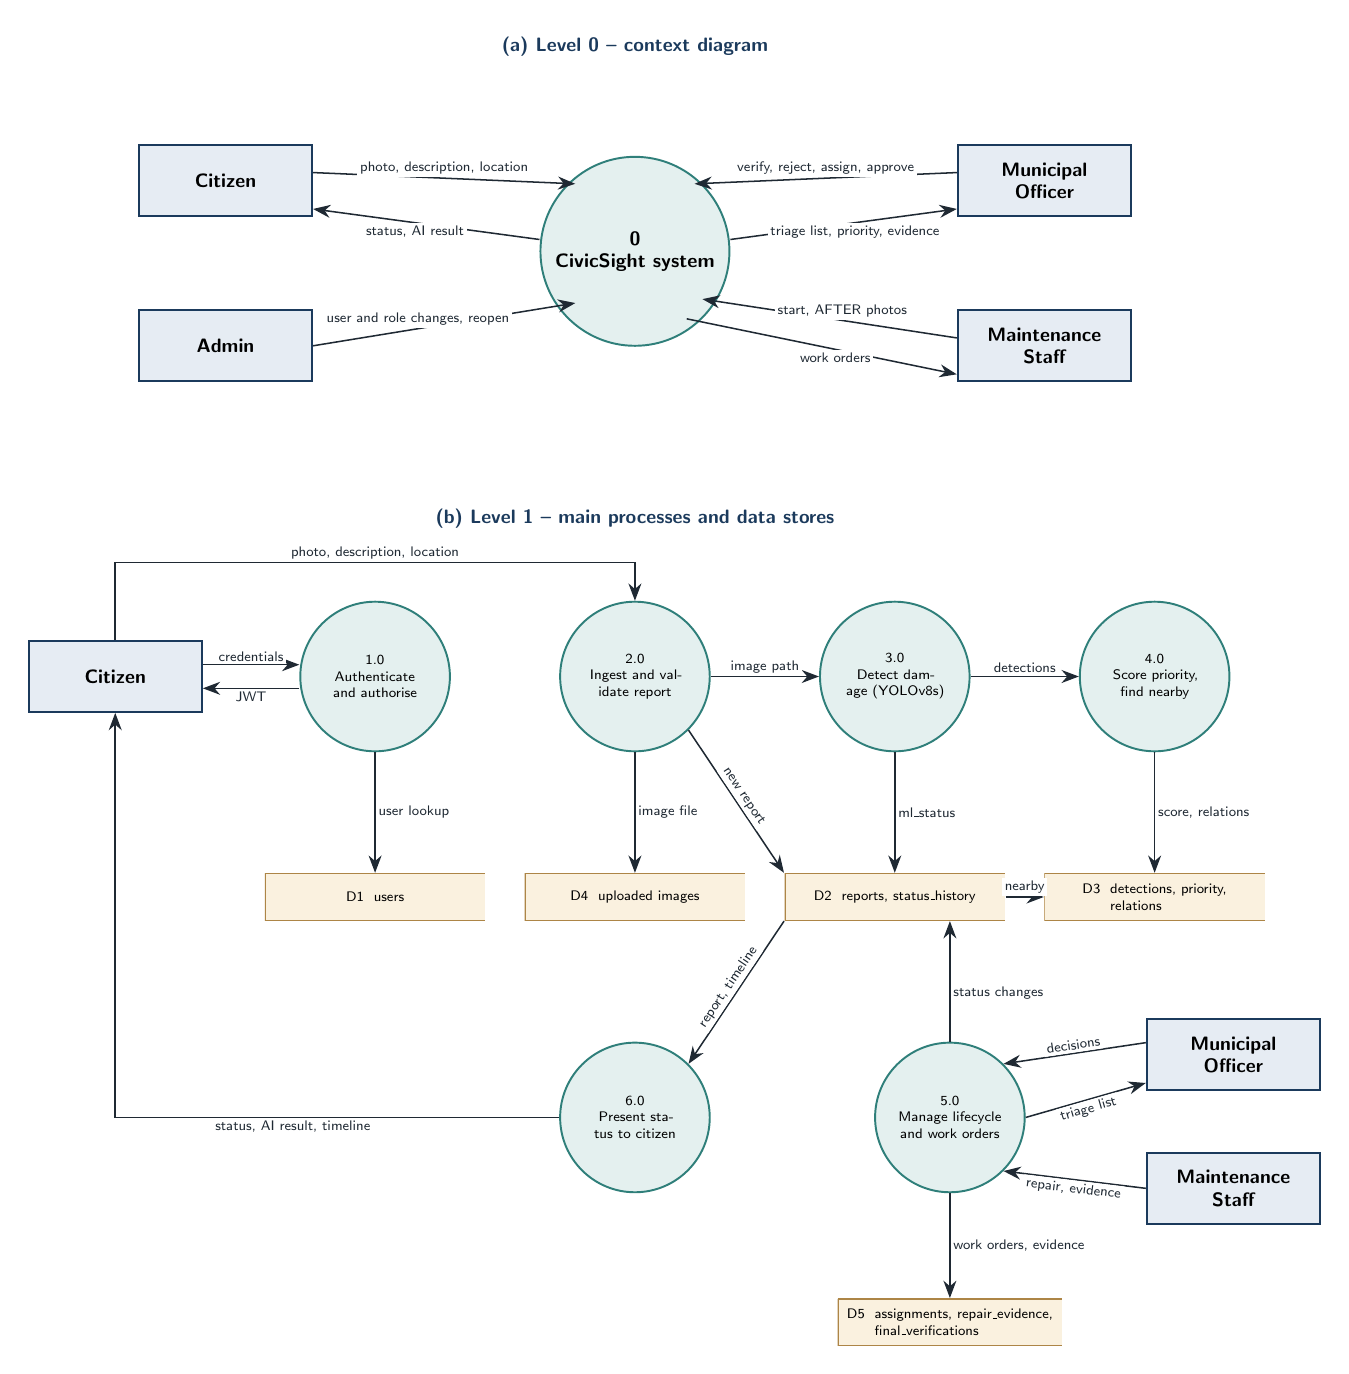
\begin{tikzpicture}[
    ext/.style={rectangle,draw=csNavy,fill=csNavyLight,line width=0.7pt,minimum width=22mm,minimum height=9mm,
      font=\sffamily\scriptsize\bfseries,align=center},
    proc/.style={circle,draw=csTeal,fill=csTealLight,line width=0.7pt,minimum size=19mm,align=center,
      font=\sffamily\tiny,inner sep=1pt,text width=17mm},
    store/.style={draw=none,minimum width=28mm,minimum height=6mm,font=\sffamily\tiny,align=left,
      path picture={\draw[csSand!80!black,line width=0.7pt] (path picture bounding box.north west) -- (path picture bounding box.north east)
      (path picture bounding box.south west) -- (path picture bounding box.south east)
      (path picture bounding box.north west) -- (path picture bounding box.south west);},fill=csSandLight},
    df/.style={->,draw=csInk,line width=0.55pt}, dl/.style={lbl,font=\sffamily\tiny,align=center}]

  % ================= Level 0 =================
  \node[font=\sffamily\scriptsize\bfseries,text=csNavy] at (0,2.6) {(a) Level 0 -- context diagram};
  \node[proc,minimum size=24mm,text width=21mm,font=\sffamily\scriptsize\bfseries] (sys) at (0,0) {0\\CivicSight system};
  \node[ext] (c) at (-5.2,0.9) {Citizen};
  \node[ext] (o) at (5.2,0.9) {Municipal\\Officer};
  \node[ext] (m) at (5.2,-1.2) {Maintenance\\Staff};
  \node[ext] (a) at (-5.2,-1.2) {Admin};
  \draw[df] ($(c.east)+(0,1mm)$) -- node[dl,above] {photo, description, location} ($(sys.north west)+(0.1,0)$);
  \draw[df] ($(sys.west)+(0,0.15)$) -- node[dl,below,pos=0.55] {status, AI result} ($(c.south east)+(0,1mm)$);
  \draw[df] ($(o.west)+(0,1mm)$) -- node[dl,above] {verify, reject, assign, approve} ($(sys.north east)+(-0.1,0)$);
  \draw[df] ($(sys.east)+(0,0.15)$) -- node[dl,below,pos=0.55] {triage list, priority, evidence} ($(o.south west)+(0,1mm)$);
  \draw[df] ($(m.west)+(0,1mm)$) -- node[dl,above,pos=0.45] {start, AFTER photos} ($(sys.south east)+(0,0.25)$);
  \draw[df] ($(sys.south east)+(-0.2,0)$) -- node[dl,below,pos=0.55] {work orders} ($(m.south west)+(0,1mm)$);
  \draw[df] (a.east) -- node[dl,above,pos=0.4] {user and role changes, reopen} ($(sys.south west)+(0.1,0.2)$);

  % ================= Level 1 =================
  \begin{scope}[yshift=-5.4cm]
  \node[font=\sffamily\scriptsize\bfseries,text=csNavy] at (0,2.0) {(b) Level 1 -- main processes and data stores};
  \node[ext] (c1) at (-6.6,0) {Citizen};
  \node[proc] (p1) at (-3.3,0) {1.0\\Authenticate and authorise};
  \node[proc] (p2) at (0,0) {2.0\\Ingest and validate report};
  \node[proc] (p3) at (3.3,0) {3.0\\Detect damage (YOLOv8s)};
  \node[proc] (p4) at (6.6,0) {4.0\\Score priority, find nearby};
  \node[store] (d1) at (-3.3,-2.8) {D1\ \ users};
  \node[store] (d4) at (0,-2.8) {D4\ \ uploaded images};
  \node[store] (d2) at (3.3,-2.8) {D2\ \ reports, status\_history};
  \node[store] (d3) at (6.6,-2.8) {D3\ \ detections, priority,\\\phantom{D3\ \ }relations};
  \node[proc] (p6) at (0,-5.6) {6.0\\Present status to citizen};
  \node[proc] (p5) at (4.0,-5.6) {5.0\\Manage lifecycle and work orders};
  \node[ext] (o1) at (7.6,-4.8) {Municipal\\Officer};
  \node[ext] (m1) at (7.6,-6.5) {Maintenance\\Staff};
  \node[store] (d5) at (4.0,-8.2) {D5\ \ assignments, repair\_evidence,\\\phantom{D5\ \ }final\_verifications};

  \draw[df] ($(c1.east)+(0,0.15)$) -- node[dl,above] {credentials} ($(p1.west)+(0,0.15)$);
  \draw[df] ($(p1.west)+(0,-0.15)$) -- node[dl,below] {JWT} ($(c1.east)+(0,-0.15)$);
  \draw[df] (p1) -- node[dl,right] {user lookup} (d1);
  \draw[df] (c1.north) |- node[dl,above,pos=0.75] {photo, description, location} (0,1.45) -- (p2.north);
  \draw[df] (p2) -- node[dl,above] {image path} (p3);
  \draw[df] (p2) -- node[dl,right] {image file} (d4);
  \draw[df] (p2.south east) -- node[dl,above,sloped] {new report} (d2.north west);
  \draw[df] (p3) -- node[dl,right] {ml\_status} (d2);
  \draw[df] (p3) -- node[dl,above] {detections} (p4);
  \draw[df] (p4) -- node[dl,right] {score, relations} (d3);
  \draw[df] (d2.east) -- node[dl,above] {nearby} (d3.west);
  \draw[df] ($(o1.west)+(0,0.15)$) -- node[dl,above,sloped] {decisions} (p5.north east);
  \draw[df] (p5.east) -- node[dl,below,sloped] {triage list} ($(o1.south west)+(0,0.1)$);
  \draw[df] (m1.west) -- node[dl,below,sloped] {repair, evidence} (p5.south east);
  \draw[df] (p5) -- node[dl,right,pos=0.4] {status changes} (d2.south -| p5);
  \draw[df] (p5) -- node[dl,right] {work orders, evidence} (d5);
  \draw[df] (d2.south west) -- node[dl,above,sloped] {report, timeline} (p6.north east);
  \draw[df] (p6.west) -| node[dl,below,pos=0.3] {status, AI result, timeline} (c1.south);
  \end{scope}
\end{tikzpicture}
%% ---- end diagrams/dfd.tex ----
}
  \caption{Data flow diagrams: (a) Level 0 context diagram, (b) Level 1 diagram}
  \label{fig:dfd}
\end{figure}

\subsection{Class Design}

Figure~\ref{fig:class} shows the nine SQLAlchemy domain classes and the core service classes.
\code{Report} is the central aggregate. It \emph{owns} its detections, status history, priority
history, assignments, repair evidence and final verifications, which are deleted with it. The lower
part shows where the business logic lives: \code{RoleChecker} for authorisation, the
\code{state\_machine} module, \code{PriorityConfig} with the scoring functions, and the ML and proximity
services.

\begin{figure}[htbp]
  \centering
  \resizebox{\linewidth}{!}{%
%% ---- begin diagrams/classdiagram.tex ----
% UML class diagram: SQLAlchemy domain model (models.py) + core/service classes
\begin{tikzpicture}[
    cls/.style={rectangle split,rectangle split parts=3,draw=csNavy,line width=0.6pt,
      rectangle split part fill={csNavyLight,white,white},align=left,inner sep=2.2pt,
      font=\sffamily\tiny,text width=#1},
    cls/.default=31mm,
    svc/.style={cls=#1,draw=csTeal,rectangle split part fill={csTealLight,white,white}},
    svc/.default=31mm,
    enm/.style={rectangle split,rectangle split parts=2,draw=csSand!80!black,line width=0.6pt,
      rectangle split part fill={csSandLight,white},align=left,inner sep=2.2pt,font=\sffamily\tiny,text width=24mm},
    assoc/.style={draw=csInk,line width=0.55pt},
    comp/.style={draw=csInk,line width=0.55pt,{Diamond[length=2.6mm,width=1.8mm]}-},
    dep/.style={draw=csSlate,line width=0.55pt,dashed,->},
    m/.style={font=\sffamily\tiny,text=csTerra,inner sep=1pt}]
  %

  % ------------------- core entities -------------------
  \node[cls=36mm] (rep) at (0,0) {\cn{Report}
    \nodepart{second}+ id: int\\+ description: str\\+ latitude, longitude: float\\+ image\_url: str\\
      + status: ReportStatus\\+ priority, severity: str\\+ priority\_score: float\\+ ml\_status: str\\
      + nearby\_report\_count: int\\+ version: int (optimistic lock)\\+ duplicate\_of\_id: int [0..1]
    \nodepart{third}+ status\_history: list\\+ detection\_results: list\\+ assignments: list\\+ repair\_evidence: list};
  \node[cls=31mm,above=10mm of rep] (usr) {\cn{User}
    \nodepart{second}+ id: int\\+ name, email, phone: str\\+ hashed\_password: str\\+ role: UserRole\\+ is\_active: bool
    \nodepart{third}+ reports: list[Report]};
  \node[enm,left=12mm of usr] (role) {\centering\textbf{\guillemotleft enum\guillemotright\ UserRole}
    \nodepart{second}CITIZEN\\MUNICIPAL\_OFFICER\\MAINTENANCE\_STAFF\\ADMIN};
  \node[enm,text width=34mm,right=12mm of usr] (rstat) {\centering\textbf{\guillemotleft enum\guillemotright\ ReportStatus}
    \nodepart{second}SUBMITTED, PENDING\_VERIFICATION, VERIFIED, ASSIGNED, UNDER\_REPAIR,
      REPAIR\_EVIDENCE\_SUBMITTED, CLOSED, REJECTED, DUPLICATE};

  % left column
  \node[cls=31mm,left=14mm of rep.north west,anchor=north east] (det) {\cn{DetectionResult}
    \nodepart{second}+ detected\_class: str\\+ confidence: float\\+ bbox\_xmin..bbox\_ymax: float\\+ severity, model\_version: str
    \nodepart{third}};
  \node[cls=31mm,below=4mm of det] (his) {\cn{ReportStatusHistory}
    \nodepart{second}+ from\_status, to\_status: str\\+ performed\_by\_id: int\\+ performed\_by\_role: str\\+ note: str
    \nodepart{third}};
  \node[cls=31mm,below=4mm of his] (pri) {\cn{PriorityHistory}
    \nodepart{second}+ previous/new\_priority: str\\+ score: float\\+ trigger: str
    \nodepart{third}};

  % right column
  \node[cls=31mm,right=14mm of rep.north east,anchor=north west] (asg) {\cn{Assignment}
    \nodepart{second}+ assigned\_to: int (User)\\+ assigned\_by: int (User)\\+ is\_active: bool\\+ unassigned\_at: datetime
    \nodepart{third}};
  \node[cls=31mm,below=4mm of asg] (evi) {\cn{RepairEvidence}
    \nodepart{second}+ kind: EvidenceKind\\+ file\_path, mime\_type: str\\+ size\_bytes: int\\+ checksum: str (SHA-256)
    \nodepart{third}};
  \node[cls=31mm,below=4mm of evi] (fin) {\cn{FinalVerification}
    \nodepart{second}+ officer\_id: int\\+ decision: VerificationDecision\\+ note: str
    \nodepart{third}};
  \node[cls=31mm,below=8mm of rep] (rel) {\cn{ReportRelation}
    \nodepart{second}+ report\_id, related\_report\_id\\+ distance\_meters: float\\+ relation\_type: str\\+ review\_status: str
    \nodepart{third}};

  % compositions (Report owns its children; cascade delete)
  \draw[comp] (rep.west |- det.east) -- node[m,above,pos=0.85] {0..*} node[m,above,pos=0.1] {1} (det.east);
  \draw[comp] ($(rep.west)+(0,-6mm)$) -| ($(his.east)+(5mm,0)$) -- node[m,above,pos=0.6] {0..*} (his.east);
  \draw[comp] ($(rep.south west)+(4mm,0)$) |- node[m,above,pos=0.92] {0..*} (pri.east);
  \draw[comp] (rep.east |- asg.west) -- node[m,above,pos=0.85] {0..*} node[m,above,pos=0.1] {1} (asg.west);
  \draw[comp] ($(rep.east)+(0,-6mm)$) -| ($(evi.west)+(-5mm,0)$) -- node[m,above,pos=0.6] {0..*} (evi.west);
  \draw[comp] ($(rep.south east)+(-4mm,0)$) |- node[m,above,pos=0.92] {0..*} (fin.west);
  \draw[comp] (rep.south) -- node[m,right,pos=0.8] {0..*} (rel.north);
  % associations with User
  \draw[assoc] (usr.south) -- node[m,right,pos=0.15] {0..1 reporter} node[m,right,pos=0.85] {0..*} (rep.north);
  \draw[dep] (usr.west) -- node[lbl,above] {uses} (role.east);
  \draw[dep] (rep.north east) -- node[lbl,above,sloped] {uses} (rstat.south west);

  % ------------------- services / core -------------------
  \node[svc=38mm,below=14mm of rel,xshift=-44mm] (rc) {\cn{RoleChecker}
    \nodepart{second}- allowed\_roles: list[str]
    \nodepart{third}+ \_\_call\_\_(current\_user): User\\\quad raises 403 if role not allowed};
  \node[svc=38mm,right=6mm of rc.north east,anchor=north west] (sm) {\cn{\guillemotleft module\guillemotright\ state\_machine}
    \nodepart{second}+ LEGAL\_TRANSITIONS: dict\\+ ROLE\_TRANSITIONS: dict
    \nodepart{third}+ validate\_transition(cur, tgt,\\\quad role, is\_assigned\_staff)};
  \node[svc=38mm,right=6mm of sm.north east,anchor=north west] (pc) {\cn{PriorityConfig}
    \nodepart{second}+ class\_weights: dict\\+ min\_confidence = 0.25\\+ high/medium thresholds
    \nodepart{third}+ calculate\_severity(dets)\\+ calculate\_priority(...): dict};
  \node[svc=38mm,below=5mm of rc] (mls) {\cn{\guillemotleft service\guillemotright\ ml\_service}
    \nodepart{second}+ INFERENCE\_TIMEOUT = 30 s
    \nodepart{third}+ process\_report\_image\_ml(id)\\+ run\_ml\_inference\_guarded(path)};
  \node[svc=38mm,below=5mm of sm] (prox) {\cn{\guillemotleft service\guillemotright\ proximity}
    \nodepart{second}+ NEARBY = 50 m, DUPLICATE = 15 m
    \nodepart{third}+ haversine\_distance(...)\\+ process\_report\_proximity(r)};
  \node[svc=38mm,below=5mm of pc] (ad) {\cn{\guillemotleft module\guillemotright\ inference\_adapter}
    \nodepart{second}+ CLASS\_METADATA (4 classes)\\- \_MODEL\_CACHE: dict
    \nodepart{third}+ detect\_road\_damage(img, conf, iou)};
  \draw[dep] (mls.east) -- node[lbl,above] {calls} (prox.west);
  \draw[dep] (prox.east) -- node[lbl,above] {calls} (ad.west |- prox.east);
  \draw[dep] (mls.south) -- ++(0,-9mm) -| node[lbl,pos=0.25,below] {inference} (ad.south);
  \draw[dep] (prox.north) -- node[lbl,right] {scores via} (pc.south west);
\end{tikzpicture}
%% ---- end diagrams/classdiagram.tex ----
}
  \caption{UML class diagram (domain model and core services)}
  \label{fig:class}
\end{figure}

\subsection{Database Design}

The database has nine tables (Figure~\ref{fig:erd}). The \code{reports} table holds the \emph{current}
state of each report, while every change is written to append-only history tables. This keeps
dashboard queries fast and the audit trail complete. Integrity is enforced in the database itself:
foreign keys are switched on for every connection; child rows use \code{ON DELETE CASCADE}, while user
references use \code{SET NULL} so deleting a user never deletes reports; \code{report\_relations} has a
unique pair constraint and a no-self-link check; and composite indexes
(\code{ix\_reports\_status\_priority}, \code{ix\_reports\_lat\_lng}) serve the triage and proximity
queries. A \code{version} column provides optimistic locking: an update succeeds only if the row has not
changed since it was read, otherwise the API returns HTTP~409.

\begin{figure}[htbp]
  \centering
  \resizebox{\linewidth}{!}{%
%% ---- begin diagrams/erd.tex ----
% Entity relationship diagram (backend/app/models/models.py). PK = primary key, FK = foreign key.
%
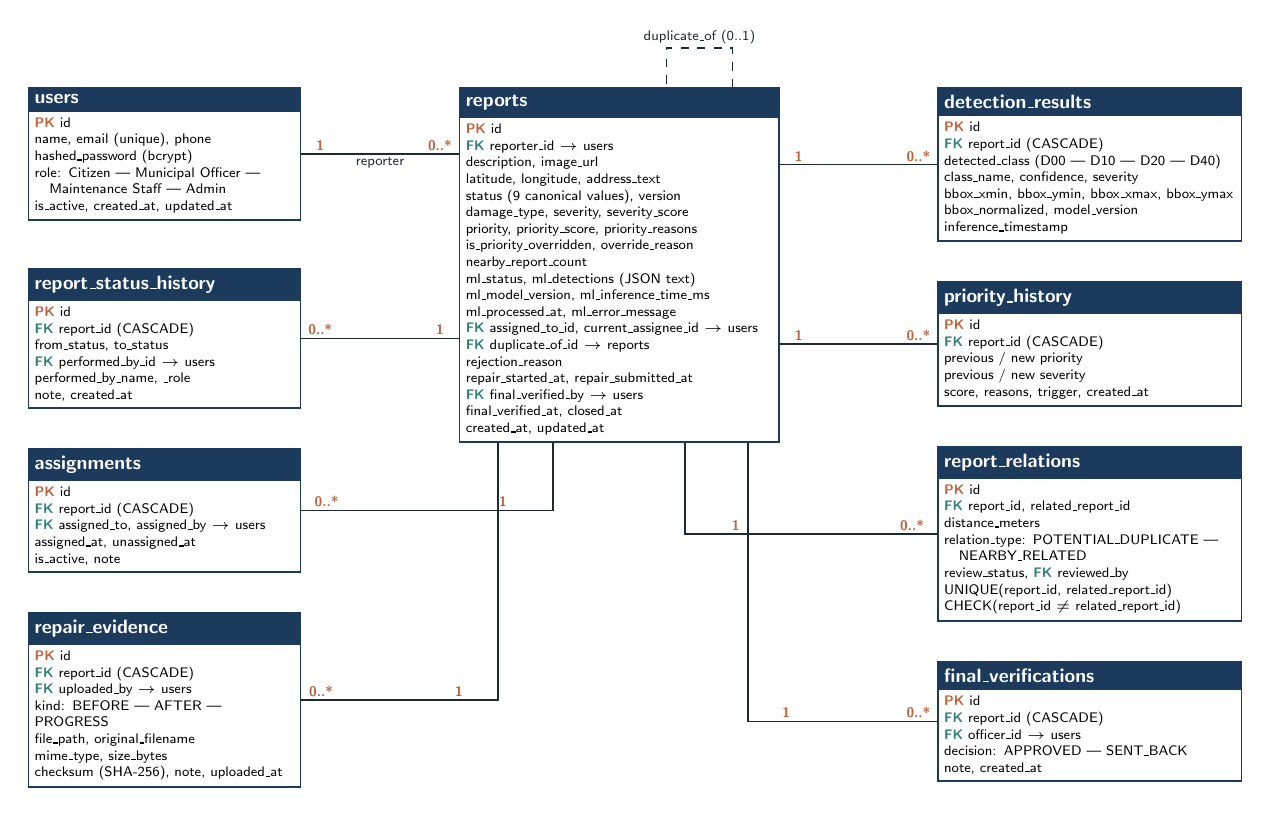
\begin{tikzpicture}[
    e/.style={rectangle split,rectangle split parts=2,draw=csNavy,line width=0.6pt,
      rectangle split part fill={csNavy,white},align=left,inner sep=2.2pt,
      font=\sffamily\tiny,text width=#1},
    rel/.style={draw=csInk,line width=0.6pt},
    one/.style={font=\sffamily\tiny\bfseries,text=csTerra,inner sep=1pt},
    pk/.style={}]
  %
  %

  % ---------------- reports (centre) ----------------
  \node[e=39mm] (rep) at (0,0) {\textcolor{white}{\textbf{\scriptsize reports}}
    \nodepart{two}\PK id\\
    \FK reporter\_id $\rightarrow$ users\\
    description, image\_url\\
    latitude, longitude, address\_text\\
    status (9 canonical values), version\\
    damage\_type, severity, severity\_score\\
    priority, priority\_score, priority\_reasons\\
    is\_priority\_overridden, override\_reason\\
    nearby\_report\_count\\
    ml\_status, ml\_detections (JSON text)\\
    ml\_model\_version, ml\_inference\_time\_ms\\
    ml\_processed\_at, ml\_error\_message\\
    \FK assigned\_to\_id, current\_assignee\_id $\rightarrow$ users\\
    \FK duplicate\_of\_id $\rightarrow$ reports\\
    rejection\_reason\\
    repair\_started\_at, repair\_submitted\_at\\
    \FK final\_verified\_by $\rightarrow$ users\\
    final\_verified\_at, closed\_at\\
    created\_at, updated\_at};

  % ---------------- users ----------------
  \node[e=33mm,left=20mm of rep.north west,anchor=north east] (usr) {\textcolor{white}{\textbf{\scriptsize users}}
    \nodepart{two}\PK id\\
    name, email (unique), phone\\
    hashed\_password (bcrypt)\\
    role: Citizen | Municipal Officer |\\\quad Maintenance Staff | Admin\\
    is\_active, created\_at, updated\_at};

  % ---------------- right column ----------------
  \node[e=37mm,right=20mm of rep.north east,anchor=north west] (det) {\textcolor{white}{\textbf{\scriptsize detection\_results}}
    \nodepart{two}\PK id\\
    \FK report\_id (CASCADE)\\
    detected\_class (D00 | D10 | D20 | D40)\\
    class\_name, confidence, severity\\
    bbox\_xmin, bbox\_ymin, bbox\_xmax, bbox\_ymax\\
    bbox\_normalized, model\_version\\
    inference\_timestamp};
  \node[e=37mm,below=5mm of det] (pri) {\textcolor{white}{\textbf{\scriptsize priority\_history}}
    \nodepart{two}\PK id\\
    \FK report\_id (CASCADE)\\
    previous / new priority\\
    previous / new severity\\
    score, reasons, trigger, created\_at};
  \node[e=37mm,below=5mm of pri] (rel) {\textcolor{white}{\textbf{\scriptsize report\_relations}}
    \nodepart{two}\PK id\\
    \FK report\_id, related\_report\_id\\
    distance\_meters\\
    relation\_type: POTENTIAL\_DUPLICATE |\\\quad NEARBY\_RELATED\\
    review\_status, \FK reviewed\_by\\
    UNIQUE(report\_id, related\_report\_id)\\
    CHECK(report\_id $\neq$ related\_report\_id)};

  % ---------------- left column (below users) ----------------
  \node[e=33mm,below=6mm of usr] (his) {\textcolor{white}{\textbf{\scriptsize report\_status\_history}}
    \nodepart{two}\PK id\\
    \FK report\_id (CASCADE)\\
    from\_status, to\_status\\
    \FK performed\_by\_id $\rightarrow$ users\\
    performed\_by\_name, \_role\\
    note, created\_at};
  \node[e=33mm,below=5mm of his] (asg) {\textcolor{white}{\textbf{\scriptsize assignments}}
    \nodepart{two}\PK id\\
    \FK report\_id (CASCADE)\\
    \FK assigned\_to, assigned\_by $\rightarrow$ users\\
    assigned\_at, unassigned\_at\\
    is\_active, note};

  % ---------------- bottom row ----------------
  \node[e=33mm,below=5mm of asg] (evi) {\textcolor{white}{\textbf{\scriptsize repair\_evidence}}
    \nodepart{two}\PK id\\
    \FK report\_id (CASCADE)\\
    \FK uploaded\_by $\rightarrow$ users\\
    kind: BEFORE | AFTER | PROGRESS\\
    file\_path, original\_filename\\
    mime\_type, size\_bytes\\
    checksum (SHA-256), note, uploaded\_at};
  \node[e=37mm,below=5mm of rel] (fin) {\textcolor{white}{\textbf{\scriptsize final\_verifications}}
    \nodepart{two}\PK id\\
    \FK report\_id (CASCADE)\\
    \FK officer\_id $\rightarrow$ users\\
    decision: APPROVED | SENT\_BACK\\
    note, created\_at};

  % ---------------- relationships ----------------
    \draw[rel] (usr.east) -- node[one,above,pos=0.12] {1} node[one,above,pos=0.88] {0..*} node[lbl,below] {reporter} (usr.east -| rep.west);
  \draw[rel] (rep.west |- his.east) -- node[one,above,pos=0.12] {1} node[one,above,pos=0.88] {0..*} (his.east);
  \draw[rel] ($(rep.south west)+(12mm,0)$) |- node[one,above,pos=0.6] {1} node[one,above,pos=0.95] {0..*} (asg.east);
  \draw[rel] (rep.east |- det.west) -- node[one,above,pos=0.12] {1} node[one,above,pos=0.88] {0..*} (det.west);
  \draw[rel] (rep.east |- pri.west) -- node[one,above,pos=0.12] {1} node[one,above,pos=0.88] {0..*} (pri.west);
  \draw[rel] ($(rep.south east)+(-12mm,0)$) |- node[one,above,pos=0.6] {1} node[one,above,pos=0.95] {0..*} (rel.west);
  \draw[rel] ($(rep.south east)+(-4mm,0)$) |- node[one,above,pos=0.6] {1} node[one,above,pos=0.95] {0..*} (fin.west);
  \draw[rel] ($(rep.south west)+(5mm,0)$) |- node[one,above,pos=0.6] {1} node[one,above,pos=0.95] {0..*} (evi.east);
  % self reference (duplicate_of_id)
  \draw[rel,dashed] ($(rep.north east)+(-6mm,0)$) -- ++(0,5mm) -| node[lbl,pos=0.25,above] {duplicate\_of (0..1)} ($(rep.north)+(6mm,0)$);
\end{tikzpicture}
%% ---- end diagrams/erd.tex ----
}
  \caption{Entity relationship diagram of the CivicSight database}
  \label{fig:erd}
\end{figure}

\subsection{Report Lifecycle State Machine}

A new report starts as SUBMITTED (Figure~\ref{fig:state}). While awaiting review it can be verified,
rejected (a reason is mandatory) or marked as a duplicate. A verified report is assigned, repaired and
submitted with evidence; the officer then closes it or sends it back for rework. Dashed arrows are
mistake-recovery paths. Officers and Admins perform review, assignment and closure; only the
\emph{assigned} staff member (or an Admin) can start a repair and submit evidence; citizens cannot change
any status; and only Admins can reopen CLOSED, REJECTED or DUPLICATE reports. Of the 324 possible
(from, to, role) combinations, exactly 34 are allowed.

\begin{figure}[htbp]
  \centering
  \adjustbox{max width=0.85\linewidth,max totalheight=0.52\textheight}{%
%% ---- begin diagrams/statemachine.tex ----
% Report lifecycle state machine (LEGAL_TRANSITIONS + ROLE_TRANSITIONS in app/core/state_machine.py)
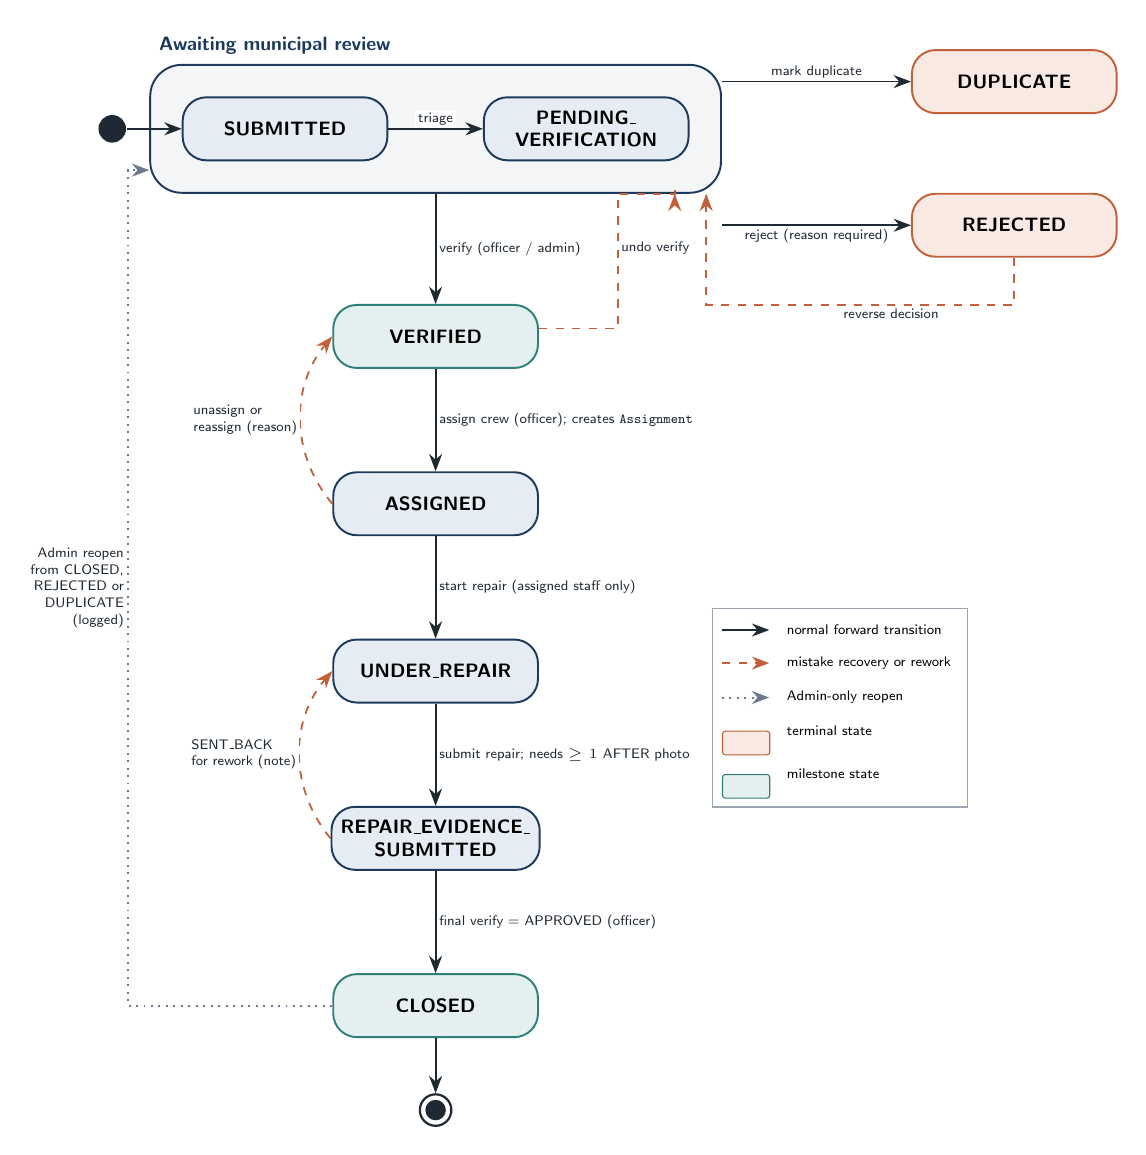
\begin{tikzpicture}[
    t/.style={->,draw=csInk,line width=0.65pt},
    tl/.style={lbl,font=\sffamily\tiny,align=left},
    rev/.style={->,draw=csTerra,line width=0.65pt,dashed},
    adm/.style={->,draw=csSlate,line width=0.7pt,dotted}]
  % composite state "awaiting review"
  \node[st] (sub) at (0,0) {SUBMITTED};
  \node[st,right=12mm of sub] (pend) {PENDING\_\\VERIFICATION};
  \node[start,left=7mm of sub] (init) {};
  \draw[t] (init) -- (sub);
  \draw[t] (sub) -- node[tl,above] {triage} (pend);
  \begin{scope}[on background layer]
    \node[draw=csNavy,fill=csLight,rounded corners=4mm,line width=0.7pt,inner sep=4mm,
          fit=(sub)(pend),label={[font=\sffamily\scriptsize\bfseries,text=csNavy,anchor=south west]north west:Awaiting municipal review}] (grp) {};
  \end{scope}

  % main spine
  \node[stok,below=14mm of grp.south] (ver) {VERIFIED};
  \node[st,below=13mm of ver] (asg) {ASSIGNED};
  \node[st,below=13mm of asg] (ur) {UNDER\_REPAIR};
  \node[st,below=13mm of ur] (res) {REPAIR\_EVIDENCE\_\\SUBMITTED};
  \node[stok,below=13mm of res] (clo) {CLOSED};
  \node[stop,below=7mm of clo] (end) {};

  % terminal side states
  \node[stterm,right=24mm of grp.east,yshift=6mm] (dup) {DUPLICATE};
  \node[stterm,below=10mm of dup] (rej) {REJECTED};

  % forward transitions
  \draw[t] (grp.south) -- node[tl,right] {verify (officer / admin)} (ver);
  \draw[t] (grp.east |- dup) -- node[tl,above] {mark duplicate} (dup);
  \draw[t] (grp.east |- rej.west) ++(0,0) -- node[tl,below] {reject (reason required)} (rej);
  \draw[t] (ver) -- node[tl,right] {assign crew (officer); creates \code{Assignment}} (asg);
  \draw[t] (asg) -- node[tl,right] {start repair (assigned staff only)} (ur);
  \draw[t] (ur) -- node[tl,right] {submit repair; needs $\geq 1$ AFTER photo} (res);
  \draw[t] (res) -- node[tl,right] {final verify = APPROVED (officer)} (clo);
  \draw[t] (clo) -- (end);

  % recovery / rework transitions
  \draw[rev] ($(ver.east)+(0,1mm)$) -- ++(10mm,0) |- node[tl,pos=0.3,right] {undo verify} ($(grp.south east)+(-6mm,0)$) -- ++(0,0);
  \draw[rev] (asg.west) to[bend left=40] node[tl,left] {unassign or\\reassign (reason)} (ver.west);
  \draw[rev] (res.west) to[bend left=40] node[tl,left] {SENT\_BACK\\for rework (note)} (ur.west);
  \draw[rev] (rej.south) -- ++(0,-6mm) -| node[tl,pos=0.2,below] {reverse decision} ($(grp.south east)+(-2mm,0)$);

  % admin reopen
  \draw[adm] (clo.west) -- ++(-26mm,0) |- node[tl,pos=0.25,left,align=right] {Admin reopen\\from CLOSED,\\REJECTED or\\DUPLICATE\\(logged)} ($(grp.south west)+(0,3mm)$);

  % legend
  \matrix[draw=csLine,fill=white,inner sep=3pt,row sep=2pt,column sep=3pt,anchor=north west]
    at ($(ur.east)+(22mm,8mm)$) {
    \draw[t] (0,0) -- (6mm,0); & \node[anchor=west,font=\sffamily\tiny] {normal forward transition}; \\
    \draw[rev] (0,0) -- (6mm,0); & \node[anchor=west,font=\sffamily\tiny] {mistake recovery or rework}; \\
    \draw[adm] (0,0) -- (6mm,0); & \node[anchor=west,font=\sffamily\tiny] {Admin-only reopen}; \\
    \node[draw=csTerra,fill=csTerraLight,rounded corners=1pt,minimum width=6mm,minimum height=3mm] {}; & \node[anchor=west,font=\sffamily\tiny] {terminal state}; \\
    \node[draw=csTeal,fill=csTealLight,rounded corners=1pt,minimum width=6mm,minimum height=3mm] {}; & \node[anchor=west,font=\sffamily\tiny] {milestone state}; \\
  };
\end{tikzpicture}
%% ---- end diagrams/statemachine.tex ----
}
  \caption{UML state machine of a report (\code{app/core/state\_machine.py})}
  \label{fig:state}
\end{figure}

\subsection{Workflows}

Figure~\ref{fig:act-sub} shows report submission and damage detection. The citizen first gets an
instant AI preview. After submission, the server validates and stores the report, runs proximity and
priority, replies immediately, and analyses the photo in the background. Figure~\ref{fig:act-repair}
shows the municipal workflow from verification through assignment and repair to closure, including the
rework loop. Figure~\ref{fig:seq-final} details final verification. The \code{alt} fragment shows
optimistic locking: if another officer changed the report first, zero rows are updated and the API
returns HTTP~409 instead of silently overwriting that decision.

\begin{figure}[htbp]
  \centering
  \adjustbox{max width=\linewidth,max totalheight=0.66\textheight}{%
%% ---- begin diagrams/activity_submission.tex ----
% Activity diagram: citizen report submission and damage detection (report.js, reports.py, ml_service.py)
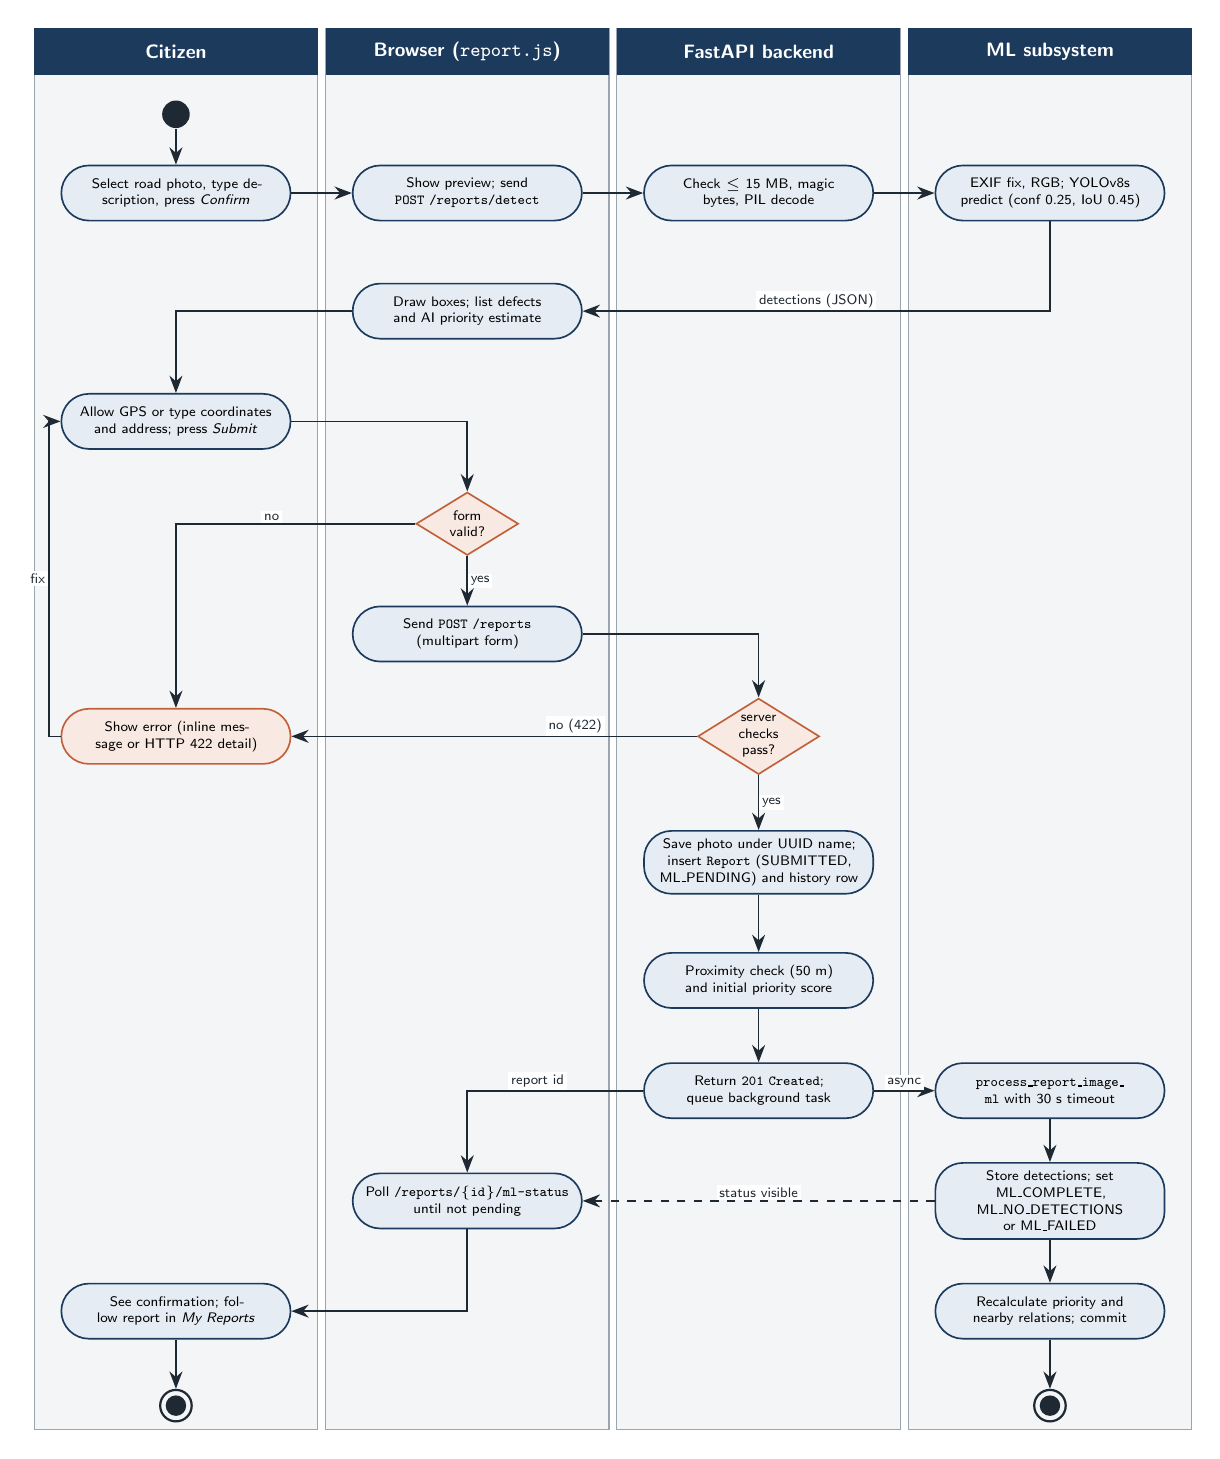
\begin{tikzpicture}[a/.style={act=27mm,font=\sffamily\tiny},
    dc/.style={decision,minimum width=13mm,minimum height=8mm},
    f/.style={flow}, fl/.style={lbl,font=\sffamily\tiny}]
  \def\LA{0} \def\LB{3.7} \def\LC{7.4} \def\LD{11.1}
  \foreach \x/\t in {\LA/Citizen,\LB/Browser (\code{report.js}),\LC/FastAPI backend,\LD/ML subsystem} {
    \node[lane,minimum width=36mm,minimum height=178mm,anchor=north] at (\x,0.6) {};
    \node[fill=csNavy,text=white,font=\sffamily\scriptsize\bfseries,minimum width=36mm,minimum height=6mm,anchor=north] at (\x,0.6) {\t};
  }
  \node[start] (s) at (\LA,-0.5) {};
  \node[a] (c1) at (\LA,-1.5) {Select road photo, type description, press \textit{Confirm}};
  \node[a] (b1) at (\LB,-1.5) {Show preview; send \code{POST /reports/detect}};
  \node[a] (k1) at (\LC,-1.5) {Check $\leq$ 15 MB, magic bytes, PIL decode};
  \node[a] (m1) at (\LD,-1.5) {EXIF fix, RGB; YOLOv8s predict (conf 0.25, IoU 0.45)};
  \node[a] (b2) at (\LB,-3.0) {Draw boxes; list defects and AI priority estimate};
  \node[a] (c2) at (\LA,-4.4) {Allow GPS or type coordinates and address; press \textit{Submit}};
  \node[dc] (cv) at (\LB,-5.7) {form\\valid?};
  \node[a] (post) at (\LB,-7.1) {Send \code{POST /reports} (multipart form)};
  \node[dc] (sv) at (\LC,-8.4) {server\\checks\\pass?};
  \node[a,draw=csTerra,fill=csTerraLight] (err) at (\LA,-8.4) {Show error (inline message or HTTP 422 detail)};
  \node[a] (save) at (\LC,-10.0) {Save photo under UUID name; insert \code{Report} (SUBMITTED, ML\_PENDING) and history row};
  \node[a] (prox) at (\LC,-11.5) {Proximity check (50 m) and initial priority score};
  \node[a] (bg) at (\LC,-12.9) {Return \code{201 Created}; queue background task};
  \node[a] (m2) at (\LD,-12.9) {\code{process\_report\_image\_ml} with 30 s timeout};
  \node[a] (poll) at (\LB,-14.3) {Poll \code{/reports/\{id\}/ml-status} until not pending};
  \node[a] (m3) at (\LD,-14.3) {Store detections; set ML\_COMPLETE, ML\_NO\_DETECTIONS or ML\_FAILED};
  \node[a] (m4) at (\LD,-15.7) {Recalculate priority and nearby relations; commit};
  \node[a] (done) at (\LA,-15.7) {See confirmation; follow report in \textit{My Reports}};
  \node[stop] (e) at (\LA,-16.9) {};
  \node[stop] (e2) at (\LD,-16.9) {};

  \draw[f] (s) -- (c1);
  \draw[f] (c1) -- (b1);
  \draw[f] (b1) -- (k1);
  \draw[f] (k1) -- (m1);
  \draw[f] (m1.south) |- node[fl,pos=0.75,above] {detections (JSON)} (b2.east);
  \draw[f] (b2.west) -| (c2.north);
  \draw[f] (c2.east) -| (cv.north);
  \draw[f] (cv.south) -- node[fl,right] {yes} (post);
  \draw[f] (cv.west) -| node[fl,pos=0.3,above] {no} (err.north);
  \draw[f] (post.east) -| (sv.north);
  \draw[f] (sv.west) -- node[fl,above,pos=0.3] {no (422)} (err.east);
  \draw[f] (err.west) -- ++(-1.5mm,0) |- node[fl,pos=0.25,left] {fix} (c2.west);
  \draw[f] (sv.south) -- node[fl,right] {yes} (save);
  \draw[f] (save) -- (prox);
  \draw[f] (prox) -- (bg);
  \draw[f] (bg) -- node[fl,above] {async} (m2);
  \draw[f] (bg.west) -| node[fl,pos=0.3,above] {report id} (poll.north);
  \draw[f] (m2) -- (m3);
  \draw[f] (m3) -- (m4);
  \draw[dflow] (m3.west) -- node[fl,above] {status visible} (poll.east);
  \draw[f] (poll.south) |- (done.east);
  \draw[f] (done) -- (e);
  \draw[f] (m4) -- (e2);
\end{tikzpicture}
%% ---- end diagrams/activity_submission.tex ----
}
  \caption{Activity diagram: report submission and damage detection}
  \label{fig:act-sub}
\end{figure}

\begin{figure}[htbp]
  \centering
  \adjustbox{max width=\linewidth,max totalheight=0.66\textheight}{%
%% ---- begin diagrams/activity_repair.tex ----
% Activity diagram: municipal verification, assignment, maintenance and closure (reports.py lifecycle endpoints)
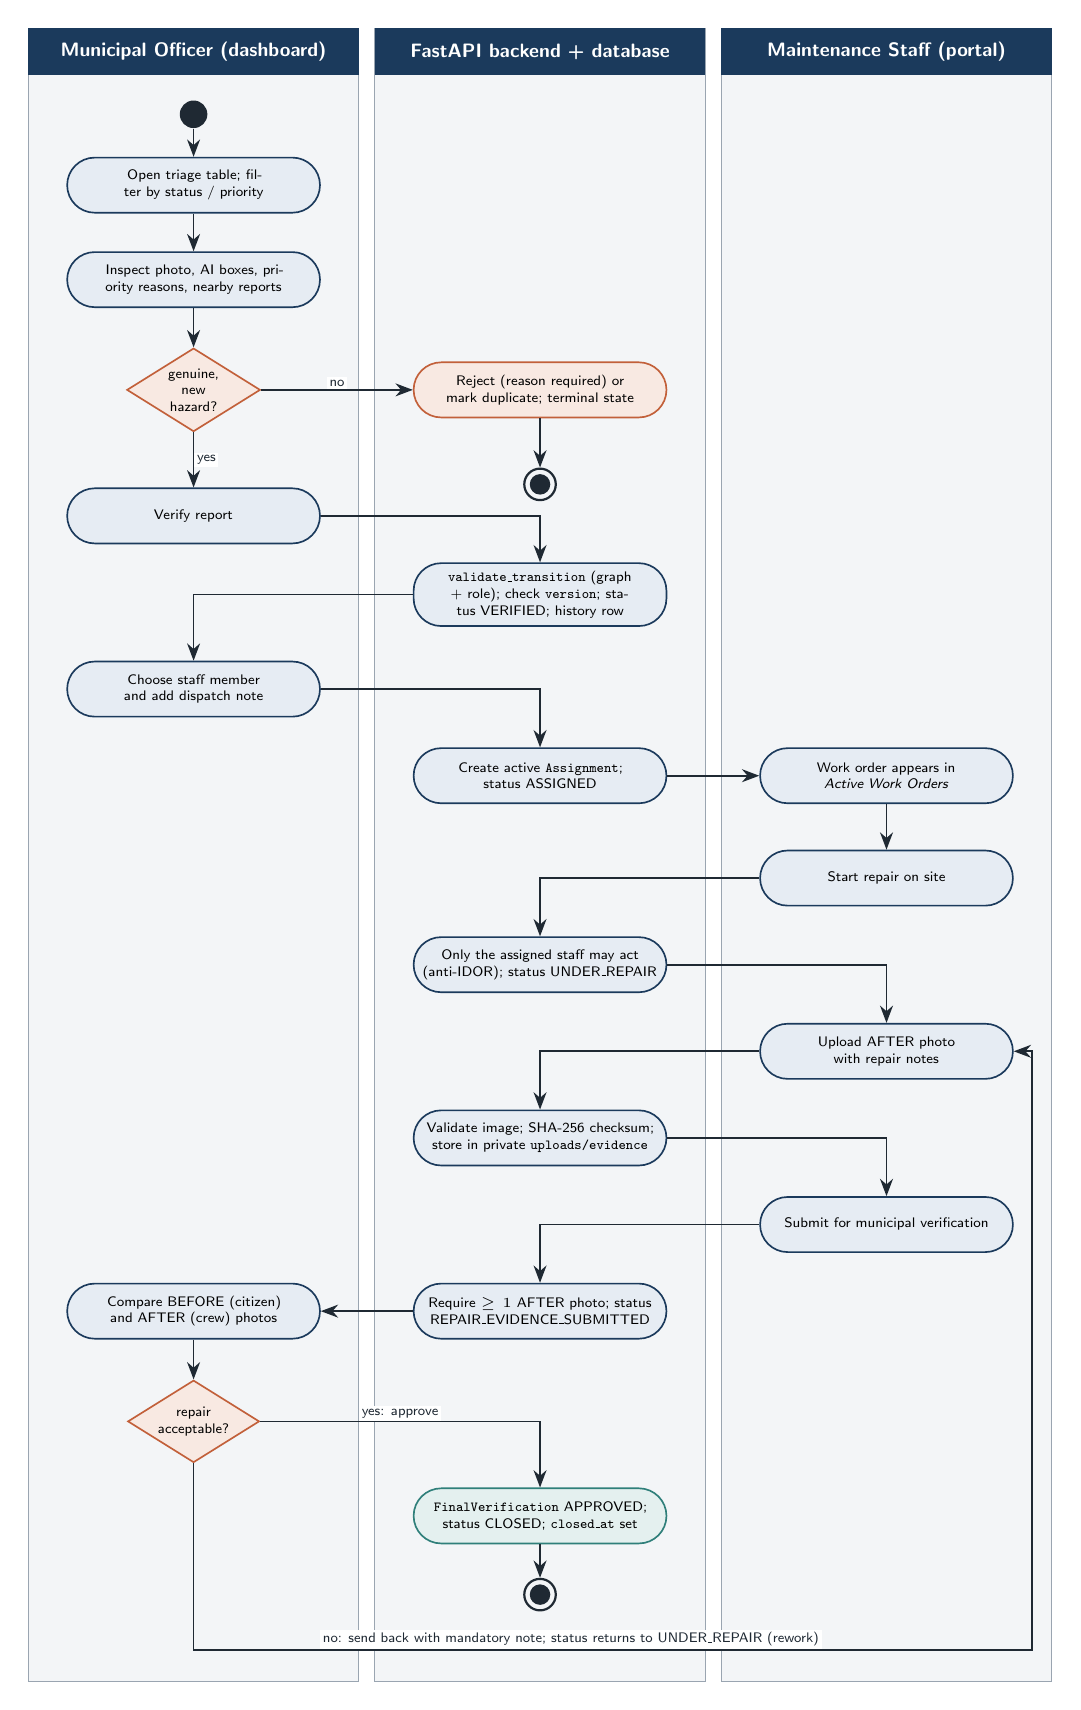
\begin{tikzpicture}[a/.style={act=30mm,font=\sffamily\tiny},
    dc/.style={decision,minimum width=13mm,minimum height=8mm},
    f/.style={flow}, fl/.style={lbl,font=\sffamily\tiny}]
  \def\LA{0} \def\LB{4.4} \def\LC{8.8}
  \foreach \x/\t in {\LA/Municipal Officer (dashboard),\LB/FastAPI backend + database,\LC/Maintenance Staff (portal)} {
    \node[lane,minimum width=42mm,minimum height=210mm,anchor=north] at (\x,0.6) {};
    \node[fill=csNavy,text=white,font=\sffamily\scriptsize\bfseries,minimum width=42mm,minimum height=6mm,anchor=north] at (\x,0.6) {\t};
  }
  \node[start] (s) at (\LA,-0.5) {};
  \node[a] (o1) at (\LA,-1.4) {Open triage table; filter by status / priority};
  \node[a] (o2) at (\LA,-2.6) {Inspect photo, AI boxes, priority reasons, nearby reports};
  \node[dc] (d1) at (\LA,-4.0) {genuine,\\new\\hazard?};
  \node[a,draw=csTerra,fill=csTerraLight] (rj) at (\LB,-4.0) {Reject (reason required) or mark duplicate; terminal state};
  \node[stop] (e1) at (\LB,-5.2) {};
  \node[a] (o3) at (\LA,-5.6) {Verify report};
  \node[a] (k1) at (\LB,-6.6) {\code{validate\_transition} (graph + role); check \code{version}; status VERIFIED; history row};
  \node[a] (o4) at (\LA,-7.8) {Choose staff member and add dispatch note};
  \node[a] (k2) at (\LB,-8.9) {Create active \code{Assignment}; status ASSIGNED};
  \node[a] (s1) at (\LC,-8.9) {Work order appears in \textit{Active Work Orders}};
  \node[a] (s2) at (\LC,-10.2) {Start repair on site};
  \node[a] (k3) at (\LB,-11.3) {Only the assigned staff may act (anti-IDOR); status UNDER\_REPAIR};
  \node[a] (s3) at (\LC,-12.4) {Upload AFTER photo with repair notes};
  \node[a] (k4) at (\LB,-13.5) {Validate image; SHA-256 checksum; store in private \code{uploads/evidence}};
  \node[a] (s4) at (\LC,-14.6) {Submit for municipal verification};
  \node[a] (k5) at (\LB,-15.7) {Require $\geq 1$ AFTER photo; status REPAIR\_EVIDENCE\_SUBMITTED};
  \node[a] (o5) at (\LA,-15.7) {Compare BEFORE (citizen) and AFTER (crew) photos};
  \node[dc] (d2) at (\LA,-17.1) {repair\\acceptable?};
  \node[a,draw=csTeal,fill=csTealLight] (k6) at (\LB,-18.3) {\code{FinalVerification} APPROVED; status CLOSED; \code{closed\_at} set};
  \node[stop] (e2) at (\LB,-19.3) {};

  \draw[f] (s) -- (o1);
  \draw[f] (o1) -- (o2);
  \draw[f] (o2) -- (d1);
  \draw[f] (d1.east) -- node[fl,above] {no} (rj.west);
  \draw[f] (rj) -- (e1);
  \draw[f] (d1) -- node[fl,right] {yes} (o3);
  \draw[f] (o3.east) -| (k1.north);
  \draw[f] (k1.west) -| (o4.north);
  \draw[f] (o4.east) -| (k2.north);
  \draw[f] (k2) -- (s1);
  \draw[f] (s1) -- (s2);
  \draw[f] (s2.west) -| (k3.north);
  \draw[f] (k3.east) -| (s3.north);
  \draw[f] (s3.west) -| (k4.north);
  \draw[f] (k4.east) -| (s4.north);
  \draw[f] (s4.west) -| (k5.north);
  \draw[f] (k5) -- (o5);
  \draw[f] (o5) -- (d2);
  \draw[f] (d2.east) -| node[fl,pos=0.25,above] {yes: approve} (k6.north);
  \draw[f] (k6) -- (e2);
  \draw[f] (d2.south) -- (\LA,-20.0) -- node[fl,above,pos=0.45] {no: send back with mandatory note; status returns to UNDER\_REPAIR (rework)} (\LC+1.85,-20.0) |- (s3.east);
\end{tikzpicture}
%% ---- end diagrams/activity_repair.tex ----
}
  \caption{Activity diagram: municipal verification, assignment, maintenance and closure}
  \label{fig:act-repair}
\end{figure}

\begin{figure}[htbp]
  \centering
  \resizebox{0.95\linewidth}{!}{%
%% ---- begin diagrams/seq_finalverify.tex ----
% Sequence diagram: final verification with optimistic locking (dashboard.js, reports.py final_verify_report)
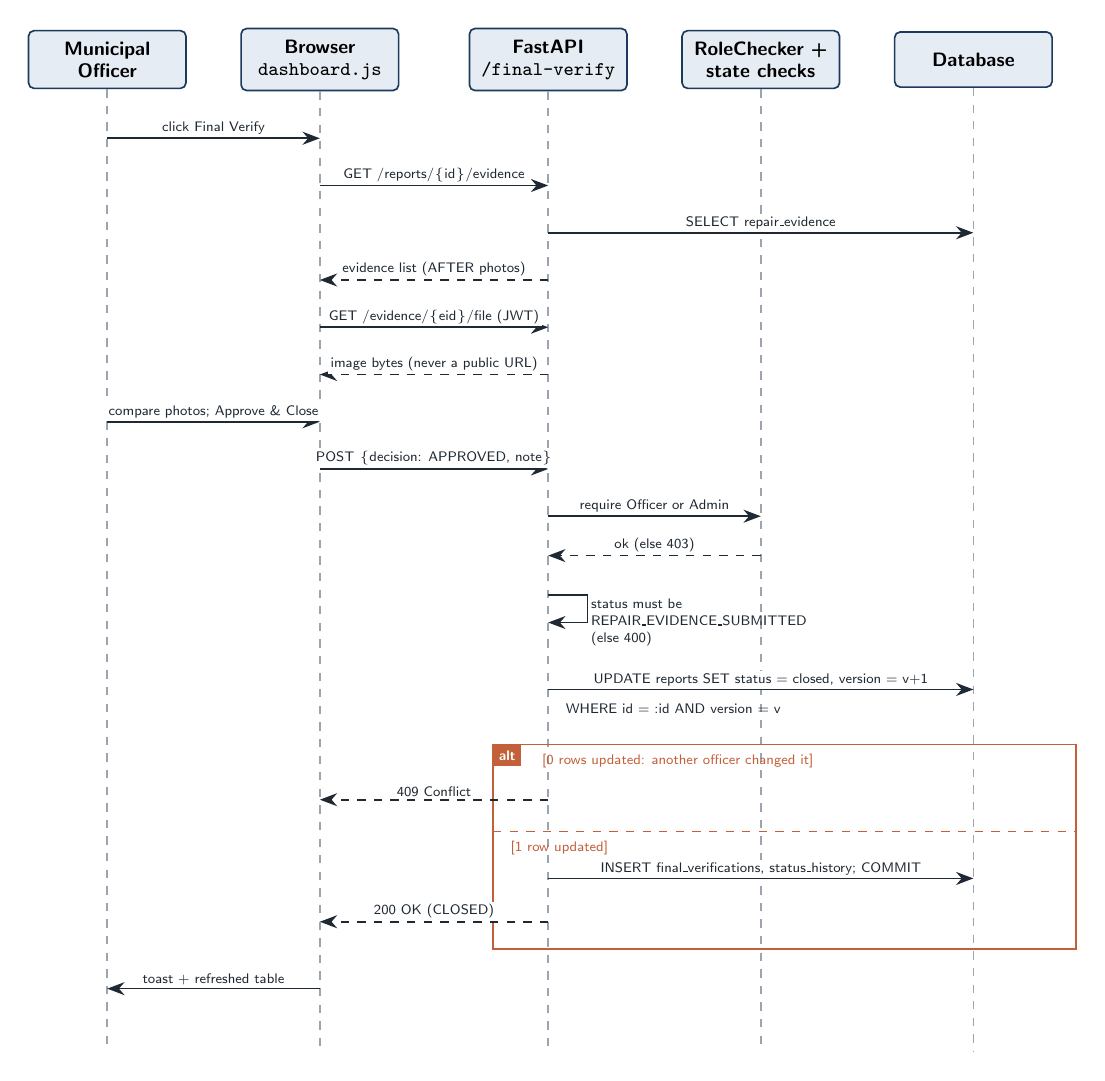
\begin{tikzpicture}
  \seqactor{off}{0}{Municipal\\Officer}
  \seqactor{br}{2.7}{Browser\\\code{dashboard.js}}
  \seqactor{api}{5.6}{FastAPI\\\code{/final-verify}}
  \seqactor{rc}{8.3}{RoleChecker +\\state checks}
  \seqactor{db}{11.0}{Database}
  \foreach \n in {off,br,api,rc,db} \seqline{\n}{-12.6};

  \msg{off}{br}{-1.0}{click Final Verify}
  \msg{br}{api}{-1.6}{GET /reports/\{id\}/evidence}
  \msg{api}{db}{-2.2}{SELECT repair\_evidence}
  \rmsg{api}{br}{-2.8}{evidence list (AFTER photos)}
  \msg{br}{api}{-3.4}{GET /evidence/\{eid\}/file (JWT)}
  \rmsg{api}{br}{-4.0}{image bytes (never a public URL)}
  \msg{off}{br}{-4.6}{compare photos; Approve \& Close}
  \msg{br}{api}{-5.2}{POST \{decision: APPROVED, note\}}
  \msg{api}{rc}{-5.8}{require Officer or Admin}
  \rmsg{rc}{api}{-6.3}{ok (else 403)}
  \selfmsg{api}{-6.8}{status must be\\REPAIR\_EVIDENCE\_SUBMITTED\\(else 400)}
  \msg{api}{db}{-8.0}{UPDATE reports SET status = closed, version = v+1}
  \node[font=\sffamily\tiny,text=csInk,anchor=west] at (5.7,-8.25) {WHERE id = :id AND version = v};

  % alt frame
  \draw[csTerra,line width=0.6pt] (4.9,-8.7) rectangle (12.3,-11.3);
  \node[fill=csTerra,text=white,font=\sffamily\tiny\bfseries,anchor=north west,inner sep=2pt] at (4.9,-8.7) {alt};
  \node[font=\sffamily\tiny,anchor=north west,text=csTerra] at (5.4,-8.7) {[0 rows updated: another officer changed it]};
  \rmsg{api}{br}{-9.4}{409 Conflict}
  \draw[csTerra,dashed] (4.9,-9.8) -- (12.3,-9.8);
  \node[font=\sffamily\tiny,anchor=north west,text=csTerra] at (5.0,-9.8) {[1 row updated]};
  \msg{api}{db}{-10.4}{INSERT final\_verifications, status\_history; COMMIT}
  \rmsg{api}{br}{-10.95}{200 OK (CLOSED)}
  \msg{br}{off}{-11.8}{toast + refreshed table}
\end{tikzpicture}
%% ---- end diagrams/seq_finalverify.tex ----
}
  \caption{Sequence diagram: final verification with optimistic locking}
  \label{fig:seq-final}
\end{figure}

\needspace{10\baselineskip}
\section{Implementation Details}

\subsection{Module 1: Authentication and Role-Based Access}

Passwords are hashed with \code{bcrypt.gensalt()} (random salt, cost 12). Login issues an HS256 JWT whose
subject is the user id, with the role, name and a 24-hour expiry; the signing key comes from the
environment. Authentication (\code{get\_current\_user}) and authorisation (\code{RoleChecker}) are separate
FastAPI dependencies, and each endpoint declares the roles it accepts in its signature:

\begin{lstlisting}[language=Python]
def final_verify_report(report_id: int, body: FinalVerificationRequest,
    current_user: User = Depends(require_roles(UserRole.MUNICIPAL_OFFICER, UserRole.ADMIN)), ...):
\end{lstlisting}

Role checks are combined with \textbf{object-level (anti-IDOR) checks}: a report can be read only by
officers, admins, its owner or its assigned staff member; reporter contact details are hidden from
non-owners; and repair endpoints require the caller to be the current assignee. Login always runs a
bcrypt comparison, using a dummy hash for unknown e-mails, so response timing does not reveal which
e-mails are registered.

\subsection{Module 2: Report Submission and Validation}

\code{POST /reports} validates on the server even though the browser validates too: the description is
trimmed and limited to 2,000 characters; coordinates must be finite and in range; the photo type is
detected from its first bytes and decoded by Pillow, so a renamed text file, an empty file or a PDF is
rejected with HTTP~422. The reporter is taken from the token, not from the form. The photo is saved
under a random UUID name (immune to path traversal) and deleted again if the database insert fails.
The report and its first history row are committed together; then proximity and priority run and
the ML task is queued. When the citizen confirms the description, \code{report.js} sends the photo to
\code{/reports/detect} and \code{ml-viewer.js} draws the returned boxes (Figure~\ref{fig:ss-report}).

\begin{figure}[htbp]
  \centering
  \begin{subfigure}[t]{0.56\linewidth}\centering\shot{screenshots/report_empty}\caption{Report Damage page}\end{subfigure}\hfill
  \begin{subfigure}[t]{0.40\linewidth}\centering\shot{screenshots/report_ai_results}\caption{AI preview of a pothole photo}\end{subfigure}
  \caption{Citizen reporting with the live AI preview (real YOLOv8s output: D40 at 51\%, 129~ms on CPU)}
  \label{fig:ss-report}
\end{figure}

\subsection{Module 3: Machine Learning Implementation}

\textbf{Dataset.} The detector was trained on RDD2022~\cite{arya2022rdd2022}, road images from Japan,
India, the Czech Republic, Norway, the United States and China. CivicSight uses exactly four classes:
\textbf{D00} longitudinal crack (along the traffic direction), \textbf{D10} transverse crack (across the
lane), \textbf{D20} alligator crack (a network of joined cracks indicating base failure) and
\textbf{D40} pothole. RDD2022's ``Repair'' label marks road that has already been fixed, so it was
removed when the data was prepared. The final run used a cleaned re-split of 37,230 training, 3,286
validation and 3,285 test images. The training boxes are imbalanced: 16,607 D00, 7,725 D10, 6,819 D20
and only 4,173 D40.

\textbf{Model and training.} YOLO is a single-stage detector: one network pass predicts box positions
and classes together, which makes it fast enough for CPU use~\cite{redmon2016yolo}. Two early CPU
experiments with YOLOv8n (3.0~M parameters, about 250 images, 2--3 epochs) reached only 0.034 and 0.118
mAP50. The production model is YOLOv8s (11.1~M parameters, confirmed by loading \code{best.pt}),
initialised from weights pre-trained on the COCO dataset. Table~\ref{tab:train} lists its settings,
and Figure~\ref{fig:curves} plots its real training log.

\begin{table}[htbp]
\centering
\caption{Training configuration of the production model (from \code{args.yaml})}
\label{tab:train}
\small
\altrows
\begin{tabular}{L{3.8cm}L{10.0cm}}
\headrow \hd{Setting} & \hd{Value} \\
Model, input, batch, epochs & YOLOv8s (COCO pre-trained), 640 $\times$ 640, 16, 50 (patience 15) \\
Optimiser & AdamW, learning rate 0.001 with cosine decay to 1\%, 3 warm-up epochs \\
Augmentation & Mosaic (off for last 10 epochs), mixup 0.1, copy-paste 0.1, HSV jitter, scale, flips, RandAugment, random erasing \\
Hardware and time & NVIDIA RTX 4060 Laptop GPU, mixed precision; 15,287~s ($\approx$ 4.2 h) \\
Output & \code{best.pt}, 21.5~MiB, classes \{0: D00, 1: D10, 2: D20, 3: D40\} \\
\end{tabular}
\end{table}

\begin{figure}[htbp]
  \centering
  \includegraphics[width=\linewidth]{charts/training_curves}
  \caption{Training progress of YOLOv8s (from \code{results.csv}); the step at epoch 41 is where mosaic augmentation is switched off}
  \label{fig:curves}
\end{figure}

\textbf{Inference and integration.} The backend calls the model through \code{inference\_adapter.py}. It
loads the weights once per path and device and caches them, falls back from CUDA to CPU, runs
\code{predict} with confidence 0.25, NMS IoU 0.45 and size 640, maps class ids to D00--D40, and converts
boxes back to original-image pixels. \code{preprocess.py} corrects EXIF orientation (so portrait phone
photos are not analysed sideways), converts any colour mode to RGB and letterboxes to 640~$\times$~640.
\code{process\_report\_image\_ml} runs in a background task with a 30-second timeout and always ends in
ML\_COMPLETE (detections stored), ML\_NO\_DETECTIONS or ML\_FAILED (error stored, report kept). Priority
and proximity are then recalculated. Figure~\ref{fig:mlpipe} connects training with this online use.

\begin{figure}[htbp]
  \centering
  \resizebox{\linewidth}{!}{%
%% ---- begin diagrams/ml_pipeline.tex ----
% ML training + inference integration workflow (ml/, backend/app/services/ml_service.py, priority.py)
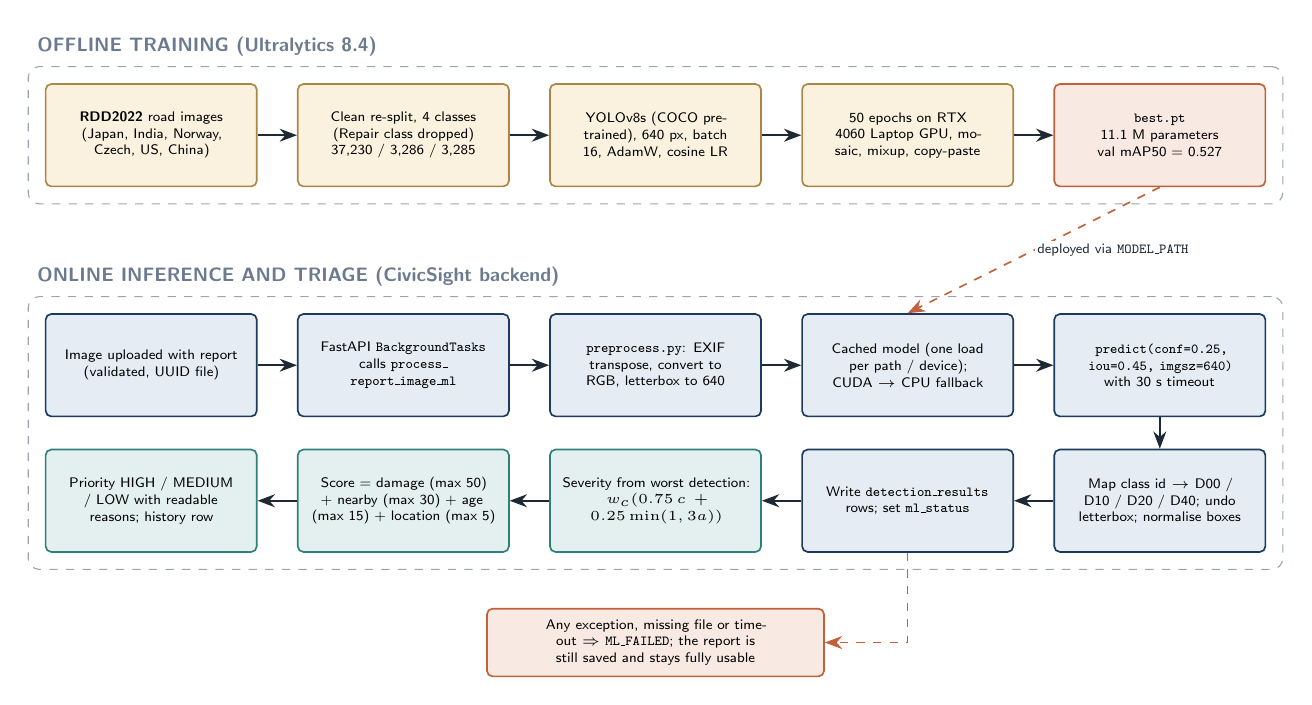
\begin{tikzpicture}[node distance=4mm and 5mm,
    p/.style={box,text width=24mm,minimum height=13mm,font=\sffamily\tiny},
    q/.style={tbox,text width=24mm,minimum height=13mm,font=\sffamily\tiny},
    r/.style={sbox,text width=24mm,minimum height=13mm,font=\sffamily\tiny}]
  % ---------------- offline training ----------------
  \node[r] (t1) {\textbf{RDD2022} road images\\(Japan, India, Norway, Czech, US, China)};
  \node[r,right=of t1] (t2) {Clean re-split, 4 classes\\(Repair class dropped)\\37,230 / 3,286 / 3,285};
  \node[r,right=of t2] (t3) {YOLOv8s (COCO pre-trained), 640 px, batch 16, AdamW, cosine LR};
  \node[r,right=of t3] (t4) {50 epochs on RTX 4060 Laptop GPU, mosaic, mixup, copy-paste};
  \node[r,right=of t4,draw=csTerra,fill=csTerraLight] (t5) {\code{best.pt}\\11.1 M parameters\\val mAP50 = 0.527};
  \foreach \a/\b in {t1/t2,t2/t3,t3/t4,t4/t5} \draw[flow] (\a) -- (\b);
  \begin{scope}[on background layer]
    \node[layer,fit=(t1)(t5),label={[layerlabel,anchor=south west]north west:OFFLINE TRAINING (Ultralytics 8.4)}] (off) {};
  \end{scope}

  % ---------------- online inference ----------------
  \node[p,below=16mm of t1] (i1) {Image uploaded with report (validated, UUID file)};
  \node[p,right=of i1] (i2) {FastAPI \code{BackgroundTasks} calls \code{process\_report\_image\_ml}};
  \node[p,right=of i2] (i3) {\code{preprocess.py}: EXIF transpose, convert to RGB, letterbox to 640};
  \node[p,right=of i3] (i4) {Cached model (one load per path / device); CUDA $\rightarrow$ CPU fallback};
  \node[p,right=of i4] (i5) {\code{predict(conf=0.25, iou=0.45, imgsz=640)} with 30 s timeout};
  \node[p,below=of i5] (i6) {Map class id $\rightarrow$ D00 / D10 / D20 / D40; undo letterbox; normalise boxes};
  \node[p,left=of i6] (i7) {Write \code{detection\_results} rows; set \code{ml\_status}};
  \node[q,left=of i7] (i8) {Severity from worst detection:\\$w_c(0.75\,c + 0.25\min(1,3a))$};
  \node[q,left=of i8] (i9) {Score = damage (max 50) + nearby (max 30) + age (max 15) + location (max 5)};
  \node[q,left=of i9] (i10) {Priority HIGH / MEDIUM / LOW with readable reasons; history row};
  \foreach \a/\b in {i1/i2,i2/i3,i3/i4,i4/i5,i5/i6,i6/i7,i7/i8,i8/i9,i9/i10} \draw[flow] (\a) -- (\b);
  \begin{scope}[on background layer]
    \node[layer,fit=(i1)(i5)(i6)(i10),label={[layerlabel,anchor=south west]north west:ONLINE INFERENCE AND TRIAGE (CivicSight backend)}] (on) {};
  \end{scope}
  \draw[flow,dashed,csTerra] (t5.south) -- node[lbl,right] {deployed via \code{MODEL\_PATH}} (t5.south |- i4.north -| i4.north) ;
  \node[rbox,text width=40mm,below=7mm of i8,font=\sffamily\tiny] (fail) {Any exception, missing file or timeout $\Rightarrow$ \code{ML\_FAILED}; the report is still saved and stays fully usable};
  \draw[dflow,csTerra] (i7.south) |- (fail.east);
\end{tikzpicture}
%% ---- end diagrams/ml_pipeline.tex ----
}
  \caption{ML training and inference integration workflow}
  \label{fig:mlpipe}
\end{figure}

\subsection{Module 4: Priority Engine and Proximity Analysis}
\label{sec:priority}

\code{priority.py} is a pure module with no database or HTTP code. Each detection with confidence
$c \geq 0.25$ gets a score $s = w_{\text{class}}\,(0.75\,c + 0.25\min(1, 3a))$, where $a$ is the box
area as a fraction of the image (at least 0.01) and the class weights are D40~1.00, D20~0.85, D10~0.55
and D00~0.40. The worst detection sets the severity: HIGH if $s \geq 0.55$, MEDIUM if $s \geq 0.28$,
otherwise LOW (UNKNOWN if ML failed). The total score adds a damage component $D$ (up to 50 points),
7.5 points per nearby report (up to 30), 1 point per day open (up to 15) and an optional location risk
(up to 5). The priority is HIGH if the severity is HIGH, at least 4 reports lie within 50~m, or the
score is at least 60; MEDIUM if the severity is MEDIUM, at least 2 reports lie nearby, or the score is
at least 30; otherwise LOW. Every rule that fires adds a plain-language reason, and officer overrides
are kept and logged.

\begin{keybox}[title=Worked example (demo report \#1).]
A pothole (D40) detected with $c = 0.51$ and a tiny box gives $s = 1.00 \times (0.3825 + 0.0075) =
0.39$, so severity is MEDIUM and $D = 28 + 8 \times 0.39 = 31.12$. A second citizen reported the same
pothole 8.8~m away, adding 7.5 points: score $= 38.62$, priority \textbf{MEDIUM}, with the reasons
``Pothole detected at 51\% confidence'' and ``1 other report within 50 m''. This matches the value
stored by the running system.
\end{keybox}

\code{proximity.py} computes distances with the Haversine formula~\cite{sinnott1984haversine}, after
pre-selecting candidates inside a latitude/longitude bounding box that uses the index. Rejected reports
are ignored. A report within 50~m becomes NEARBY\_RELATED; within 15~m and with the same (or a similar
crack) class, it becomes POTENTIAL\_DUPLICATE. Officers review the link, and neighbours' priorities are
recalculated when a new report arrives.

\subsection{Module 5: Municipal Operations and Maintenance}

The officer's dashboard (Figure~\ref{fig:ss-dash}) shows summary cards, a map panel and the triage
table with status and priority filters. Action buttons follow the status: \emph{Verify},
\emph{Assign Crew}, \emph{Reassign}/\emph{Unassign} and \emph{Final Verify}. Reports \#1 and \#2,
the same pothole reported twice, carry a \emph{Review} badge because they were linked as a potential
duplicate. The map uses the Google Maps API when a key is configured; the capture machine had no key,
so the dashboard shows its built-in fallback and the rest works normally. \emph{Inspect AI}
(Figure~\ref{fig:ss-officer}a) shows every box with the model version and timing, and states that the
AI result is decision support, not official verification. Assignment (Figure~\ref{fig:ss-officer}b)
checks that the chosen user is active Maintenance Staff and creates an \code{Assignment} record.

\begin{figure}[htbp]
  \centering
  \shot[0.86\linewidth]{screenshots/dashboard_triage_table}
  \caption{Incident triage table of the Municipal Operations Center}
  \label{fig:ss-dash}
\end{figure}

\begin{figure}[htbp]
  \centering
  \begin{subfigure}[t]{0.56\linewidth}\centering\shot{screenshots/officer_inspect_ai}\caption{Damage inspection (report \#6)}\end{subfigure}\hfill
  \begin{subfigure}[t]{0.40\linewidth}\centering\shot{screenshots/officer_assign_modal}\caption{Assign Maintenance Crew}\end{subfigure}
  \caption{Officer review and crew assignment}
  \label{fig:ss-officer}
\end{figure}

Staff see only their own work orders (\code{/staff/me/assignments}, Figure~\ref{fig:ss-staff}a). Evidence
photos are validated like report photos, checksummed with SHA-256 and stored in \code{uploads/evidence},
which is deliberately \emph{not} a public folder: images are served only through an endpoint that checks
the caller's role and assignment. Final verification (Figure~\ref{fig:ss-staff}b) places the citizen's
BEFORE photo next to the crew's AFTER photo. \emph{Approve} records a \code{FinalVerification} and closes
the report; \emph{Send Back} requires a note and returns it to UNDER\_REPAIR. Citizens follow progress on
\emph{Track My Reports} (Figure~\ref{fig:ss-my}), which loads only their own reports
(\code{/reports/mine}) and shows statuses in plain language, AI summaries and rejection reasons.

\begin{figure}[htbp]
  \centering
  \begin{subfigure}[t]{0.47\linewidth}\centering\shot{screenshots/staff_evidence_modal}\caption{Staff evidence upload}\end{subfigure}\hfill
  \begin{subfigure}[t]{0.49\linewidth}\centering\shot{screenshots/officer_final_verify_modal}\caption{Final verification: BEFORE vs AFTER}\end{subfigure}
  \caption{Repair evidence and photo-verified closure}
  \label{fig:ss-staff}
\end{figure}

\begin{figure}[htbp]
  \centering
  \shot[0.80\linewidth]{screenshots/my_reports}
  \caption{Track My Reports: counters, filters and report cards for one citizen}
  \label{fig:ss-my}
\end{figure}

\subsection{Module 6: Frontend and API}

The frontend is plain HTML, CSS and JavaScript served by FastAPI; one stylesheet defines light and dark
themes, and \code{auth.js} attaches the token and keeps users on their role's pages. The API has 35
versioned paths (46 operations) under \code{/api/v1}, documented by OpenAPI at \code{/docs}. Lifecycle
actions are explicit verbs (\code{/verify}, \code{/assign}, \code{/final-verify}) with clear error
codes (400, 401, 403, 409, 422) and no stack traces.
%% ---- end chapters/02_methodology_design.tex ----


% ===== CHAPTER 3: RESULTS & EVALUATION =====
%
%% ---- begin chapters/03_results.tex ----
% ===== CHAPTER 3: RESULTS & EVALUATION =====
\chapter{Results and Evaluation}
\label{ch:results}

All results below were measured on the project's own code, model and data. The automated test suites
were re-run on 22 November 2026 (Windows 11, Python 3.14.8, PyTorch 2.14.1 CPU build).

\section{Testing Methodology}

\begin{itemize}
  \item \textbf{Unit Testing:} pure functions were tested directly: priority bands and rules,
    Haversine distances, and the state machine. The state machine was checked \emph{exhaustively}: all
    $9 \times 9$ status pairs for each of the 4 roles (324 combinations) matched the specification.
  \item \textbf{Integration Testing:} FastAPI's \code{TestClient} sent real HTTP requests to the full
    application backed by a temporary database. These tests covered authentication, file validation,
    the full lifecycle, concurrency, evidence privacy and the real YOLOv8s model. An authorisation
    matrix checked 35 API paths against 7 identities (245 checks).
  \item \textbf{Performance Testing:} a database with 2,000 seeded reports was used to time the listing
    and proximity queries and inspect their query plans; inference was timed on CPU.
  \item \textbf{User Testing:} Playwright drove a real browser through role guards, form validation,
    themes, responsive layouts (48 page/viewport combinations) and five complete scenarios. For this
    report, the full citizen $\rightarrow$ officer $\rightarrow$ staff $\rightarrow$ officer workflow
    was run again on the live application.
\end{itemize}

\textbf{Results.} The Week~10 quality-gate suites (\code{tests/test\_week10\_backend.py} with 11 test
functions and \code{tests/test\_week10\_ml.py} with 6) \textbf{passed 17 of 17} in 47.5~s, with
\textbf{75\% statement coverage} of the backend and ML code (\code{auth.py} 100\%, \code{models.py} 96\%,
\code{state\_machine.py} 89\%, \code{reports.py} 59\%). Table~\ref{tab:tc} lists representative cases.
The older weekly test files in \code{backend/} gave 43 passed, 5 failed and 2 errors. Every failure was
an outdated expectation, not a defect: a test that expects a corrupt image to be \emph{accepted} (it has
returned 422 since Week~10), calls to \code{/reports/detect} without a login, an old error message, and
a live-server test that timed out while the CPU was busy. The Playwright suite was not re-run because
its file was being edited; its Week~10 evidence records no layout overflow, no console errors and no
unlabelled inputs.

\begin{table}[htbp]
\centering
\caption{Representative test cases with expected and actual results}
\label{tab:tc}
\small
\altrows
\begin{tabular}{C{1.1cm}L{6.4cm}L{3.6cm}L{1.6cm}C{1.1cm}}
\headrow \hd{ID} & \hd{Input / action} & \hd{Expected} & \hd{Actual} & \hd{Status} \\
TC-01 & Public registration requesting role ``Admin'' & 403, no account & 403 & \pass \\
TC-02 & Wrong password / unknown e-mail & 401, same message & 401 / 401 & \pass \\
TC-03 & Tampered or expired token on \code{/auth/me} & 401 & 401 & \pass \\
TC-04 & Text file renamed \code{.jpg}; image over 15 MB & 422 & 422 & \pass \\
TC-05 & File named \code{../../etc/passwd.jpg} (valid JPEG) & 201, stored under UUID name & as expected & \pass \\
TC-06 & SQL-injection string as status filter & 422 & 422 & \pass \\
TC-07 & Citizen opens another citizen's report & 403 & 403 & \pass \\
TC-08 & Unassigned staff member starts a repair & 403 & 403 & \pass \\
TC-09 & Illegal transition UNDER\_REPAIR $\rightarrow$ CLOSED & 400 & 400 & \pass \\
TC-10 & Submit repair without an AFTER photo & 400 & 400 & \pass \\
TC-11 & Two officers verify the same report at once & one 200, other 400/409 & one winner & \pass \\
TC-12 & Fetch evidence by its storage path & 404 (not public) & 404 & \pass \\
TC-13 & Clean road photo; broken model path & no detections; failed, report still closes & as expected & \pass \\
TC-14 & Same pothole reported twice, 8.8 m apart (live) & potential duplicate, +7.5 points each & as expected & \pass \\
\end{tabular}
\end{table}

\section{Performance Metrics}

\begin{table}[htbp]
\centering
\caption{Performance results summary}
\label{tab:performance}
\small
\altrows
\begin{tabular}{L{6.6cm}C{2.0cm}C{3.4cm}}
\headrow \hd{Metric} & \hd{Target} & \hd{Achieved} \\
Dashboard listing query, 2,000 reports & $< 50$ ms & 2.54 ms (index used) \\
Proximity query, 2,000 reports & $< 50$ ms & 0.99 ms (covering index) \\
Inference, 160 held-out road images (CPU) & $< 500$ ms & mean 130 ms, p95 170 ms \\
Inference, 16 edge-case images (CPU) & $< 500$ ms & mean 216 ms, p95 224 ms \\
Test-set precision / recall & -- & 0.608 / 0.510 \\
Test-set mAP50 / mAP50-95 & -- & 0.547 / 0.271 \\
Quality-gate tests passing & 100\% & 17 / 17 \\
\end{tabular}
\end{table}

\subsection{Machine Learning Evaluation}

\begin{keybox}[title=Metrics in plain words.]
A prediction is \emph{correct} if its box overlaps a real damage box of the same class enough, measured
by \textbf{IoU} (shared area divided by combined area). \textbf{Precision} = correct predictions
$\div$ all predictions (``when it says pothole, how often is it right?''). \textbf{Recall} = correct
predictions $\div$ all real damages (``how many potholes did it find?''). \textbf{AP} is the area under
one class's precision--recall curve~\cite{everingham2010pascal}. \textbf{mAP50} averages AP over the
four classes with IoU $\geq$ 0.5. \textbf{mAP50-95} averages over stricter IoU thresholds from 0.50 to
0.95, so it also rewards tight boxes and is always lower.
\end{keybox}

\begin{table}[htbp]
\centering
\caption{Detection metrics of the production YOLOv8s model}
\label{tab:mlmetrics}
\small
\altrows
\begin{tabular}{L{5.0cm}C{2.4cm}C{2.4cm}}
\headrow \hd{Metric} & \hd{Validation} & \hd{Test} \\
Precision / Recall & 0.596 / 0.502 & 0.608 / 0.510 \\
mAP50 / mAP50-95 (all classes) & 0.527 / 0.263 & 0.547 / 0.271 \\
\midrule
Longitudinal crack D00 (mAP50) & 0.544 & 0.539 \\
Transverse crack D10 (mAP50) & 0.498 & 0.535 \\
Alligator crack D20 (mAP50) & 0.650 & 0.646 \\
Pothole D40 (mAP50) & 0.418 & 0.469 \\
\end{tabular}
\end{table}

Test results (3,285 images) are slightly higher than validation results (3,286 images), so the model is
not over-fitted to the data used to select it (Table~\ref{tab:mlmetrics}, Figure~\ref{fig:perclass}).
Alligator cracking is detected best because its textured patches are distinctive. Potholes are hardest:
they have the fewest training boxes and vary most in size, depth and lighting. Validation mAP50 rose
from 0.118 for the best YOLOv8n experiment to 0.527 for YOLOv8s, about 4.5 times higher, mainly
because of the full dataset and GPU training.

\begin{figure}[htbp]
  \centering
  \begin{subfigure}[t]{0.52\linewidth}\centering\includegraphics[width=\linewidth]{charts/per_class_map50}\caption{Per-class mAP50}\label{fig:perclass}\end{subfigure}\hfill
  \begin{subfigure}[t]{0.45\linewidth}\centering\includegraphics[width=\linewidth]{ml/BoxPR_curve}\caption{Precision--recall curves (validation)}\label{fig:pr}\end{subfigure}
  \caption{Per-class accuracy of the production model}
  \label{fig:mlcharts}
\end{figure}

\textbf{Operating point.} The application uses one fixed threshold (confidence 0.25). On 160
stratified images from a local RDD2022 split, counting matches at IoU $\geq$ 0.5, macro precision was
0.79 and macro recall 0.52. That local split was made independently of the training split, so some
overlap is possible, and the numbers indicate behaviour rather than form a second benchmark. Only 5 of
405 ground-truth boxes received the \emph{wrong} class. Most errors were \emph{missed} damage (193) or
extra boxes (65, mostly long cracks split into pieces). Potholes had the highest precision (0.90) but
the lowest recall (0.44): when the model reports a pothole it is usually right, but it misses more than
half. This is why CivicSight keeps an officer in the loop. Difficult inputs were handled safely: clean
roads, non-road scenes and blurry night photos produced no false damage, rotated phone photos were
corrected, and 4096-pixel and 16-pixel images did not crash. Drone images, however, were often missed
or misclassified.

\textbf{Detection examples.} Figure~\ref{fig:examples} shows one real prediction of the production
model for each class, drawn by Ultralytics with the application's settings. Up to 350 images
containing each class were sampled from the local test split. The examples were then chosen, for
clarity, among predictions that match a ground-truth box of the same class with IoU $\geq$ 0.5 and
have no unmatched extra boxes (scripts \code{select\_detection\_examples.py} and
\code{render\_detection\_examples.py}). They show what a correct
detection looks like and are \emph{not} representative of average accuracy, which is given in
Table~\ref{tab:mlmetrics}.

\begin{figure}[htbp]
  \centering
  \includegraphics[width=0.96\linewidth]{ml/detection_examples}
  \caption{Genuine YOLOv8s predictions for the four classes (confidence and IoU with the ground-truth box shown under each image)}
  \label{fig:examples}
\end{figure}

\section{Analysis}

\begin{itemize}
  \item \textbf{Did we meet the objectives?} Yes. Objectives 1, 3, 4 and 5 are verified by tests
    (Table~\ref{tab:tc}). Objective 2 is met: the model covers exactly the four classes, runs in
    about 130--220~ms per image on CPU, and never blocks a report.
  \item \textbf{Where did we exceed expectations?} Robustness and safety: exhaustive state and
    authorisation matrices, concurrency protection through optimistic locking, private evidence
    storage, and database queries about 20 times faster than the target.
  \item \textbf{Where are the results weaker?} Recall (about 0.5), especially for potholes. The AI is
    useful for sorting and highlighting reports but cannot replace an officer. The pre-submission
    preview also shows a simpler class-based priority (``High'' for the demo pothole) than the
    engine's final score (MEDIUM, 38.62), and the two should be unified.
  \item \textbf{End-to-end verification.} On a fresh demo database, seven reports around Patiala went
    through real inference (six ML\_COMPLETE, one ML\_NO\_DETECTIONS for a clean road). A duplicate
    pothole was linked automatically, reports were verified, rejected and assigned, and repairs were
    evidenced and closed. The citizen's tracking page showed every state correctly.
  \item \textbf{Challenges and resolutions.} The early model was too weak (mAP50 0.03--0.12), so we
    moved to the full dataset, a GPU and YOLOv8s. RDD2022's extra ``Repair'' label was removed and the
    class ids were remapped, and a test now checks the class names stored in the weights. Inference
    that blocked uploads was moved to a timed background task. Status logic that was scattered across
    endpoints was centralised. Concurrent officer actions were made safe with optimistic locking.
    Evidence photos, which were initially public, were moved to private storage. And a missing map API
    key now falls back to manual coordinates.
  \item \textbf{Defect found during final verification.} The Assign, Reassign, Unassign and Final
    Verify dialogs opened invisibly from the dashboard table because of a missing \code{</div>} in
    \code{dashboard.html}; the API-level tests could not see this. The tag was added. Two smaller
    issues in the assign dialog (a wrong workload field name and a missing default selection) were
    also fixed, and dispatching from the default selection was verified in the browser.
\end{itemize}
%% ---- end chapters/03_results.tex ----


% ===== CHAPTER 4: CONCLUSION =====
%
%% ---- begin chapters/04_conclusion.tex ----
% ===== CHAPTER 4: CONCLUSION =====
\chapter{Conclusion}
\label{ch:conclusion}

\section{Summary of Work}

CivicSight replaces slow, informal reporting of road damage with a traceable, evidence-based
workflow. A citizen can report damage with a photo and location in under a minute. A YOLOv8s model
trained on 37,230 RDD2022 images analyses the photo, and the report is scored and de-duplicated
automatically. Officers and crews are guided through verification, assignment, repair and
photo-verified closure, while one central state machine checks every transition and records it.
All five objectives (Section~\ref{sec:objectives}) were met: validated reporting; detection of exactly
four classes at test mAP50 0.547 in 130--220~ms on CPU; explainable triage; a controlled workflow in
which all 324 transition/role combinations behave as specified; and 17 of 17 quality-gate tests passing
with 75\% coverage.

\section{Key Findings}

\begin{itemize}
  \item \textbf{Finding 1:} Data mattered more than tuning. Training on the full dataset with a slightly
    larger model raised validation mAP50 from 0.118 to 0.527.
  \item \textbf{Finding 2:} The detector rarely confuses damage types (5 of 405 boxes), but it misses
    damage, especially potholes (recall 0.44). Keeping a human in the loop is necessary, not optional.
  \item \textbf{Finding 3:} Centralising business rules in small, separately tested modules made the
    system safer and easier to verify. The only significant defect found at the end was in browser
    markup, outside those modules. This shows that browser-level tests remain important.
\end{itemize}

\section{Future Work and Recommendations}

The current limitations are modest recall (especially for drone and night images), inference inside
the web server process, SQLite and local file storage, no login rate limiting or token revocation, no
notifications, and a dependency on a Google Maps key for map views. Recommended next steps:

\begin{enumerate}
  \item Fine-tune on local Indian smartphone photos, try YOLOv8m and higher resolution, and set
    per-class thresholds from the F1 curve to improve pothole recall.
  \item Use the same priority engine for the pre-submission preview and the stored report.
  \item Run the detector on AFTER photos and warn officers if damage is still detected.
  \item Move inference to a GPU worker queue, and use PostgreSQL with migrations and cloud object
    storage for a city-wide deployment.
  \item Add e-mail/SMS notifications, a public map of open and repaired hazards, rate limiting and
    HTTP-only refresh tokens.
  \item Update or retire the older weekly tests, and add a browser test that opens every dashboard
    dialog.
\end{enumerate}

\section{Final Remarks}

Building CivicSight showed us that a useful AI product is mostly good software engineering around a
model: clear requirements, a data model that keeps history, explicit rules about who may do what,
honest handling of failures, and tests that cover whole matrices of cases. The model makes triage
faster and more objective, but the workflow, the audit trail and the officer in the loop are what make
the system trustworthy. Together these form a practical basis for a municipal pilot.
%% ---- end chapters/04_conclusion.tex ----


% ===== BIBLIOGRAPHY =====
% Print bibliography with heading in TOC
\printbibliography[heading=bibintoc]

\end{document}
